\documentclass[conference]{IEEEtran}
\IEEEoverridecommandlockouts
% The preceding line is only needed to identify funding in the first footnote. If that is unneeded, please comment it out.

% ====== IEEE Standard Packages ======
\usepackage{cite}
\usepackage{amsmath,amssymb,amsfonts}
\usepackage{algorithm}
\usepackage{algpseudocode}
\usepackage{graphicx}
\usepackage{textcomp}
\usepackage{xcolor}
\usepackage{url}
\usepackage{float}    % for [H] placement
\usepackage{booktabs} % for nicer tables


% ====== Additional Packages ======
\usepackage[utf8]{inputenc}
\usepackage{subcaption}
\usepackage[section]{placeins}
\usepackage[justification=centering]{caption}
\usepackage{multirow}
\usepackage{tikz}
\usetikzlibrary{shapes, arrows, positioning, calc, shapes.geometric}

% ====== PDF Metadata ======
\def\BibTeX{{\rm B\kern-.05em{\sc i\kern-.025em b}\kern-.08em
    T\kern-.1667em\lower.7ex\hbox{E}\kern-.125emX}}

% figures live here:
\graphicspath{{figures/}}

\title{GraphSAGE‑based Multi‑Task GNN for Joint User Pairing and Power Allocation in Downlink PD‑NOMA}

%\author{
%  \IEEEauthorblockN{ Shailendra Shukla, Anisha Dwivedi, and Ramesh Ch. Mishra}
%  \IEEEauthorblockA{\textit{Dept. of Electronics and Communication Engineering} \\
%    \textit{Indian Institute of Information Technology, Senapati, Manipur, India}\\
%     shailendra@iiitmanipur.ac.in, anishas1121@iiitmanipur.ac.in, m.ramesh@iiitmanipur.ac.in}
%}

\begin{document}
\maketitle

\begin{abstract}
Power-domain non-orthogonal multiple access (PD-NOMA) is a promising technique in 5G and beyond networks for improving spectral efficiency through intelligent user pairing and power allocation. However, traditional optimization-based user pairing strategies have cubic complexity $O(N^3)$, which hinders real-time deployment in large networks. To overcome this challenge, we propose a GraphSAGE-based graph neural network (GNN) framework, termed NOMA-GNN, that reformulates user pairing as a graph representation learning problem. We generate realistic channel state information using the 3GPP TR 38.901 urban macro model and incorporate physical constraints such as successive interference cancellation (SIC) feasibility and user angular separation into the learning process. The model is trained on data from 200 diverse network scenarios (each with 500 users, totaling 100,000 training samples) and evaluated on network sizes ranging from 500 to 2000 users. Results show that NOMA-GNN achieves near-optimal throughput (95.7–96.5\% of the optimum) across all tested densities while delivering substantial speedups relative to optimal bipartite matching: 28.1× faster at 500 users, 64.0× at 1000, and 114.4× at 2000 users. The proposed solution runs in $O(N \log N)$ time, enabling practical inference times even at high user densities. The lightweight architecture (166K parameters, 650 KB footprint) is suitable for edge base station deployment, enabling scalable NOMA in dense 5G New Radio networks.
\end{abstract}

\begin{IEEEkeywords}
Power-domain NOMA, graph neural networks, GraphSAGE, user pairing, power allocation, deep learning, resource management, 5G/6G networks, SIC feasibility
\end{IEEEkeywords}

% ====== paper body ======
\section{Introduction}

With the exponential growth of 5G networks and the imminent evolution toward 6G systems, the modern wireless landscape faces significant challenges in sustaining massive device connectivity while maximizing spectral efficiency. Power-domain non-orthogonal multiple access (PD-NOMA) has emerged as a promising technique to address these requirements. Unlike conventional orthogonal multiple access (OMA), where users occupy exclusive time–frequency resources, PD-NOMA allows multiple users to share the same resource block through power-domain multiplexing, thereby improving spectrum utilization and enhancing cell-edge performance.

The core idea of PD-NOMA is to allocate different transmit power levels according to users’ channel conditions: weaker users are assigned higher power, while stronger users receive lower power and employ successive interference cancellation (SIC) to decode and remove the weaker users’ signals. This asymmetric design enables simultaneous multi-user transmission and can significantly improve throughput and fairness, especially in dense urban deployments.

However, the performance of PD-NOMA heavily depends on \emph{user pairing}—the selection of which two users should share a physical resource block (PRB). Poor pairing choices can cause excessive inter-user interference, unsuccessful SIC decoding, and large throughput losses. Since the number of possible pairings grows combinatorially with user count, traditional optimization-based methods become computationally infeasible for real-time scheduling in large-scale 5G/6G networks. This motivates the development of scalable, learning-driven solutions capable of approximating optimal pairing with significantly lower complexity.

\section{Literature Review}

User pairing and power allocation play a pivotal role in determining the efficiency of PD-NOMA systems. Early studies approached this problem through heuristic techniques that exploited channel-gain disparity. For example, static strong–weak pairing algorithms sort users by channel magnitude and pair those at opposite ends of the list to maximize SIC feasibility, while balanced pairing splits the user set into two groups and pairs them to jointly improve fairness and throughput \cite{su2017,islam2016}. Although these methods offer low complexity and rapid decision-making, they lack adaptability in fast-fading or dense environments and can lead to suboptimal spectral efficiency.

To improve optimality, researchers formulated user pairing as a graph-based combinatorial optimization problem. Users are modeled as nodes in a graph, and potential pairings are represented as edges weighted by metrics such as achievable sum-rate, SINR gain, or fairness. Classical algorithms, including the Hungarian method \cite{kuhn1955} and Edmonds’ Blossom algorithm \cite{edmonds1965}, are then applied to extract maximum-weight matchings. Köse \textit{et al.} \cite{kose2021graph} exploited claw-free conflict graphs to simplify the computation of maximum weighted independent sets, while Jia \textit{et al.} \cite{jia2018} designed edge-weighted pairing graphs for dynamic throughput enhancement. Despite their theoretical strength, these algorithms scale poorly in real-time applications, with worst-case complexity on the order of $O(N^{3})$, making them unsuitable for large user populations.

To bridge the gap between performance and scalability, several works proposed structured matching schemes that exploit the natural strong–weak pairing pattern in NOMA. Mishra \textit{et al.} \cite{mishra2021maximizing,mishra2022connection,mishra2023globecom} introduced bipartite matching frameworks such as Minimum-Weight Full Matching with Pruning (MWFMP) and Connection Throughput Maximization with Bipartite Matching (CTMBM), enforcing strong–weak pairing under rate and latency constraints. These methods reduce computational burden and offer high throughput in practice, but they still rely on iterative optimization and repeated graph construction, which can be burdensome in rapidly time-varying channels.

In parallel, learning-based solutions have emerged to approximate optimal pairing and power allocation policies via data-driven inference. Supervised deep neural networks (DNNs) have been used to learn the mapping between user-level features (e.g., distance, path loss, SINR) and pairing or power decisions based on optimal or near-optimal training labels \cite{sun2018learning,he2020learning,eisen2020optimal}. Such models provide low inference latency and good scalability once trained. However, they typically treat users as independent inputs and ignore the relational structure of wireless interference, and they require large labeled datasets generated using computationally intensive solvers such as Blossom or bipartite matching.

To relax the dependence on labeled data and better adapt to dynamic environments, deep reinforcement learning (DRL) has also been applied to NOMA resource allocation. In this setting, user pairing and power allocation are cast as a Markov decision process, with the base station acting as an agent that learns a policy from interaction with the environment. Approaches based on deep Q-networks (DQN), dueling DQN, or deep deterministic policy gradients (DDPG) have demonstrated improved performance over purely heuristic methods in dynamic or partially observable scenarios \cite{jiang2021,hamedoon2024}. Nevertheless, DRL frameworks often suffer from long convergence times, sensitivity to hyperparameters, and performance degradation in large or high-dimensional state spaces, which complicates their deployment in large-scale networks.

Motivated by these challenges, recent research has turned toward graph neural networks (GNNs) as a natural and effective paradigm for modeling user interactions in NOMA systems. Unlike traditional DNNs, GNNs represent users as nodes and spatial or interference relationships as edges, enabling relational reasoning through message passing. The GraphSAGE model \cite{hamilton2017inductive}, in particular, supports inductive learning over varying network topologies and efficiently aggregates neighborhood features across multiple hops. Rusek \textit{et al.} \cite{rusek2020graph} showed that GNNs can predict end-to-end network performance, while Chowdhury \textit{et al.} \cite{chowdhury2021unfolding} unfolded classical optimization algorithms such as WMMSE into GNN architectures to embed physical constraints into the learning process. In the NOMA context, Jiang \textit{et al.} \cite{jiang2021} proposed NOMANet, which jointly learns user pairing and power allocation and achieves near-optimal performance with significantly reduced inference complexity compared to traditional matching algorithms.

GNN-based methods offer several advantages over earlier learning-based models. They naturally capture inter-user dependencies, can generalize across different deployment scenarios and user densities, and allow system designers to encode constraints such as SIC feasibility and angular separation directly in the graph structure or training process. Furthermore, the use of standardized channel models such as 3GPP TR~38.901 ensures that learning and evaluation are performed under realistic propagation conditions, including distance-dependent path loss, shadowing, and small-scale fading \cite{3gpp38901,etis2024}. This alignment between learning models and physical-layer constraints makes GNNs particularly attractive for deployment in dense 5G and emerging 6G networks.

Against this backdrop, the present work proposes a GraphSAGE-based GNN framework that reformulates the NOMA user pairing and power allocation problem as a graph representation learning task. The main contributions are outlined below, followed by a detailed description of the system model and methodology.

\subsection{Contributions}

This work presents a unified framework that combines classical graph-based optimization with inductive graph neural networks to achieve real-time, scalable, and interpretable user pairing in PD-NOMA systems. The main contributions are:

\begin{enumerate}
    \item \textbf{Realistic channel-aware formulation:} We generate high-fidelity CSI using the 3GPP TR~38.901 Urban Macro (UMa) model and cast NOMA user pairing as a graph-based optimization problem under practical SIC and propagation constraints.

    \item \textbf{Benchmarking of classical pairing strategies:} We implement and compare four representative pairing schemes—static, balanced, Blossom matching, and bipartite matching—within a common graph-theoretic framework, quantifying their sum-rate and complexity trade-offs under standardized CSI.

    \item \textbf{GraphSAGE-based NOMA-GNN:} We design a GraphSAGE-based GNN (NOMA-GNN) that models users as nodes with CSI-derived features and predicts pairwise compatibility scores, enforcing SIC feasibility and angular separation while achieving $O(N \log N)$ inference complexity.

    \item \textbf{Near-optimal performance with large speedups:} Extensive simulations show that NOMA-GNN attains about 96.5\% of optimal Blossom throughput with up to $40.4\times$ lower runtime and a lightweight model size suitable for edge base station deployment.
\end{enumerate}


The remainder of this paper is organized as follows. Section~II introduces the system model and channel assumptions. Section~III describes traditional user pairing strategies and their graph-matching formulations. Section~IV presents the proposed NOMA-GNN architecture and training methodology. Section~V details the simulation setup and performance evaluation. Section~VI concludes the paper and outlines directions for future work.

\section{System Model}
We consider a single-cell Urban Macrocell (UMa) scenario with a base station (BS) located at height $h_{\mathrm{BS}}$ and a cell radius $R$, as illustrated in Fig.~\ref{fig:3GPP Model}. A total of $N$ user equipments (UEs) are uniformly distributed within the cell, with each user height $h_{\mathrm{UT}}\in[1.5,22.5]$\,m. The system operates at a carrier frequency $f_c = 3.5$\,GHz. On a single physical resource block (PRB) of bandwidth $B$, the BS transmits a total power $P_{\mathrm{tot}}$, with noise power per PRB given by $N_0 B$, where $N_0$ is the noise power spectral density.
%In the downlink power-domain NOMA (PD-NOMA) system, each user $u_i \in \mathcal{U} = \{u_1, u_2, \dots, u_N\}$ experiences a complex channel coefficient $h_i \in \mathbb{C}$ capturing path loss, log-normal shadowing, and small-scale fading according to the 3GPP TR~38.901 UMa model. The corresponding channel power gain is denoted by $|h_i|^2$, which is used for both user pairing and power allocation in the NOMA transmission scheme.
\begin{figure}[t]
  \centering
  \resizebox{\columnwidth}{!}{% Urban Macrocell (UMa) System Model
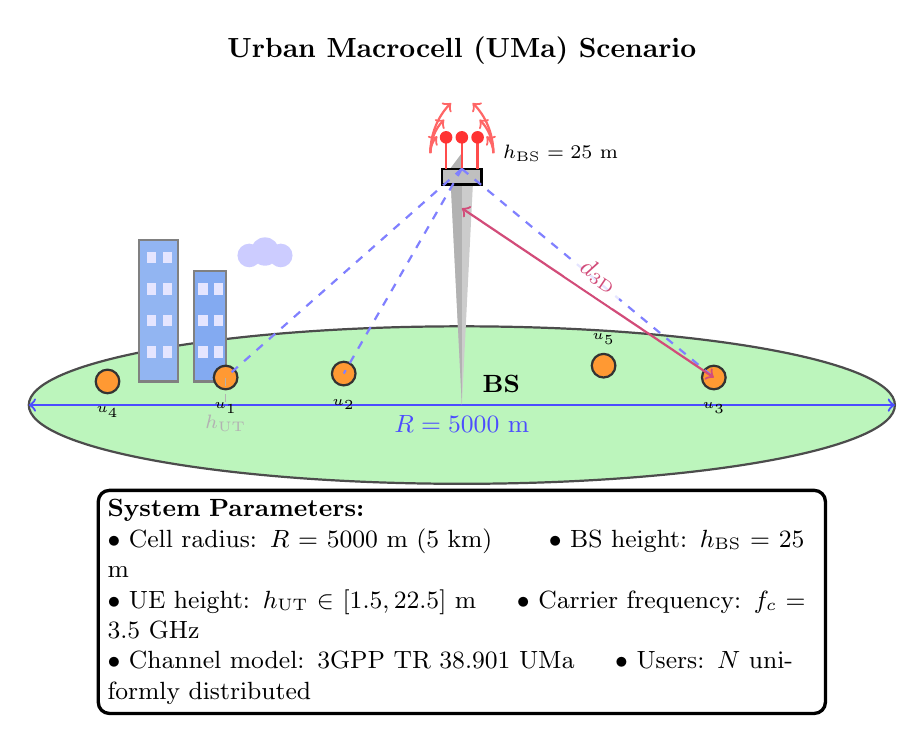
\begin{tikzpicture}[
    scale=1.0, every node/.style={scale=1.0}
]

% Define colors
\definecolor{skyblue}{RGB}{135,206,235}
\definecolor{groundgreen}{RGB}{144,238,144}
\definecolor{building}{RGB}{100,149,237}

% Ground circle (cell coverage)
\fill[groundgreen!60] (0,0) ellipse (5.5cm and 1cm);
\draw[thick, black!70] (0,0) ellipse (5.5cm and 1cm);

% Cell radius annotation
\draw[<->, thick, blue!70] (-5.5,-0) -- (5.5,-0) node[midway, below, font=\small] { $R = 5000$ m};

% Base Station Tower (CENTER)
\begin{scope}[xshift=0cm]
    % Tower structure
    \fill[gray!40] (0,0) -- (-0.15,3) -- (0.15,3) -- cycle;
    \fill[gray!60] (0,0) -- (-0.15,3) -- (0,3.2) -- cycle;
    
    % Platform at top
    \draw[fill=gray!50, thick] (-0.25,2.8) rectangle (0.25,3);
    
    % Antenna elements
    \foreach \x in {-0.2,0,0.2} {
        \draw[thick, red!70] (\x,3) -- (\x,3.4);
        \fill[red!80] (\x,3.4) circle (0.08);
    }
    
    % Signal waves
    \foreach \i in {1,2,3} {
        \draw[thick, red!60, ->] (-0.4,3.2) arc[start angle=180, end angle=135, radius=0.3*\i];
        \draw[thick, red!60, ->] (0.4,3.2) arc[start angle=0, end angle=45, radius=0.3*\i];
    }
    
    % BS label
    \node[font=\small\bfseries, below] at (0.5,0.5) {BS};
    \node[font=\scriptsize, right] at (0.4,3.2) {$h_{\mathrm{BS}} = 25$ m};
\end{scope}

% Buildings (left side)
\begin{scope}[xshift=-3.5cm, yshift=0.3cm]
    % Building 1
    \fill[building!70] (-0.6,0) rectangle (-0.1,1.8);
    \draw[thick, black!50] (-0.6,0) rectangle (-0.1,1.8);
    % Windows
    \foreach \y in {0.3,0.7,1.1,1.5} {
        \foreach \x in {-0.5,-0.3} {
            \fill[white!90!blue] (\x,\y) rectangle (\x+0.12,\y+0.15);
        }
    }
    
    % Building 2
    \fill[building!80] (0.1,0) rectangle (0.5,1.4);
    \draw[thick, black!50] (0.1,0) rectangle (0.5,1.4);
    % Windows
    \foreach \y in {0.3,0.7,1.1} {
        \foreach \x in {0.15,0.35} {
            \fill[white!90!blue] (\x,\y) rectangle (\x+0.12,\y+0.15);
        }
    }
    
    % Small cloud
    \fill[white!80!blue] (0.8,1.6) circle (0.15);
    \fill[white!80!blue] (1,1.65) circle (0.18);
    \fill[white!80!blue] (1.2,1.6) circle (0.15);
\end{scope}

% Users (UEs) distributed in cell
\begin{scope}
    % User 1 (near buildings, weak user)
    \fill[orange!80] (-3,0.35) circle (0.15);
    \draw[thick, black!80] (-3,0.35) circle (0.15);
    \node[font=\tiny, below] at (-3,0.15) {$u_1$};
    \draw[dashed, gray!60] (-3,0.35) -- (-3,0) node[below, font=\scriptsize] {$h_{\mathrm{UT}}$};
    
    % User 2 (middle-left)
    \fill[orange!80] (-1.5,0.4) circle (0.15);
    \draw[thick, black!80] (-1.5,0.4) circle (0.15);
    \node[font=\tiny, below] at (-1.5,0.2) {$u_2$};
    
    % User 3 (right, strong user) - for d3D annotation
    \fill[orange!80] (3.2,0.35) circle (0.15);
    \draw[thick, black!80] (3.2,0.35) circle (0.15);
    \node[font=\tiny, below] at (3.2,0.15) {$u_3$};
    
    % User 4 (far edge left)
    \fill[orange!80] (-4.5,0.3) circle (0.15);
    \draw[thick, black!80] (-4.5,0.3) circle (0.15);
    \node[font=\tiny, below] at (-4.5,0.1) {$u_4$};
    
    % User 5 (top right)
    \fill[orange!80] (1.8,0.5) circle (0.15);
    \draw[thick, black!80] (1.8,0.5) circle (0.15);
    \node[font=\tiny, above] at (1.8,0.65) {$u_5$};
\end{scope}

% Communication links (dashed lines from BS to users)
\draw[thick, dashed, blue!50] (0,3) -- (-3,0.35);
\draw[thick, dashed, blue!50] (0,3) -- (-1.5,0.4);
\draw[thick, dashed, blue!50] (0,3) -- (3.2,0.35);

% Distance annotations - d3D (3D distance from BS to user)
\draw[<->, thick, purple!70] (0,2.5) -- (3.2,0.35) node[midway, above, font=\small, sloped, fill=white, fill opacity=0.8, text opacity=1] {$d_{3\mathrm{D}}$};

% Title
\node[font=\normalsize\bfseries] at (0,4.5) {Urban Macrocell (UMa) Scenario};

% System parameters box
\node[draw, very thick, fill=white, rectangle, text width=90mm, font=\small, align=left, rounded corners] at (0,-2.5cm) {
\textbf{System Parameters:}\\
$\bullet$ Cell radius: $R = 5000$ m (5 km) \hspace{5mm} $\bullet$ BS height: $h_{\mathrm{BS}} = 25$ m\\
$\bullet$ UE height: $h_{\mathrm{UT}} \in [1.5, 22.5]$ m \hspace{3mm} $\bullet$ Carrier frequency: $f_c = 3.5$ GHz\\
$\bullet$ Channel model: 3GPP TR 38.901 UMa \hspace{3mm} $\bullet$ Users: $N$ uniformly distributed
};

\end{tikzpicture}
}
  \caption{Urban Macrocell (UMa) layout showing base station, distributed users, and 3GPP TR 38.901 channel model parameters.}
\end{figure}
We follow 3GPP TR~38.901 (UMa) for reproducible links \cite{etis2024}. Let $d_{2\mathrm{D}}$ be horizontal distance and $d_{3\mathrm{D}}$ the 3D distance. The UMa LOS probability is height-dependent per TR~38.901; we sample LOS/NLOS accordingly and condition subsequent large/small-scale models on that draw. For frequency in GHz and $d_{3\mathrm{D}}$ in meters, representative UMa formulas are
\begin{equation}
\mathrm{PL}_{\mathrm{LOS}}(d_{3\mathrm{D}})=28+22\log_{10}(d_{3\mathrm{D}})+20\log_{10}\!\left(\frac{f_c}{1\,\mathrm{GHz}}\right)\,\mathrm{dB}.
\end{equation}
\begin{equation}
\resizebox{\columnwidth}{!}{$
\mathrm{PL}_{\mathrm{NLOS}}(d_{3\mathrm{D}},h_{\mathrm{UT}})=13.54+39.08\log_{10}(d_{3\mathrm{D}})+20\log_{10}\!\left(\frac{f_c}{1\,\mathrm{GHz}}\right)-0.6(h_{\mathrm{UT}}-1.5)\,\mathrm{dB}.
$}
\end{equation}
Lognormal shadowing $X_\sigma\sim\mathcal{N}(0,\sigma^2)$ (in dB) is applied. The large-scale power gain is
\begin{equation}
g_{\mathrm{LS}} = 10^{-\frac{\mathrm{PL} + X_{\sigma}}{10}}.
\end{equation}
The small scale fading LOS links use Rician fading (e.g., $K\!\approx\!9$\,dB); NLOS links use Rayleigh. The composite channel magnitude obeys
\begin{equation}
|h_u| = \sqrt{g_{\mathrm{LS}}}\,\sqrt{g_{\mathrm{SS}}}, \quad |h_u|^2 = g_{\mathrm{LS}}\,g_{\mathrm{SS}}.
\end{equation}
%The base station transmits a superposed signal $x = \sum_{i\in\mathcal{U}} \sqrt{P_i}s_i$, where $s_i$ is the unit-power symbol for user $i$ and $P_i$ is the allocated transmit power. The received signal at user $i$ is
%\begin{equation}
%y_i = h_i \sum_{j\in\mathcal{U}} \sqrt{P_j}s_j + n_i,
%\end{equation}
%where $n_i \sim \mathcal{CN}(0,\sigma^2)$ is additive white Gaussian noise. 
Consider a NOMA pair $(i,j)$ on one PRB. Without loss of generality, let $i$ be the \emph{weak} user ($|h_i| < |h_j|$) and $j$ the \emph{strong} user. The total transmit power is split as
\begin{equation}
P_i = \alpha P_{\mathrm{tot}}, \qquad 
P_j = (1 - \alpha) P_{\mathrm{tot}}, \qquad 
\alpha \in (0,1),
\end{equation}
where the weak user typically receives more power (i.e., $\alpha > 0.5$).
The weak user treats the strong user’s signal as interference:
\begin{equation}
\mathrm{SINR}_i(\alpha) = 
\frac{\alpha P_{\mathrm{tot}} |h_i|^2}
{(1 - \alpha) P_{\mathrm{tot}} |h_i|^2 + N_0 B}.
\end{equation}
The strong user first decodes user $i$ (for SIC operation):
\begin{equation}
\mathrm{SINR}_{j \leftarrow i}(\alpha) =
\frac{\alpha P_{\mathrm{tot}} |h_j|^2}
{(1 - \alpha) P_{\mathrm{tot}} |h_j|^2 + N_0 B}.
\end{equation}
After cancelling $i$’s signal, the strong user decodes its own data interference-free:
\begin{equation}
\mathrm{SINR}_j(\alpha) =
\frac{(1 - \alpha) P_{\mathrm{tot}} |h_j|^2}{N_0 B}.
\end{equation}
Let $\Gamma_i$ denote the SNR (linear scale) required to support user $i$’s target rate, and let $\Delta_{\min}$ (in dB) be the practical SIC margin. The SIC constraint is satisfied if
\begin{equation}
10 \log_{10}\!\big(1 + \mathrm{SINR}_{j \leftarrow i}(\alpha)\big)
\ge
10 \log_{10}\!\big(1 + \Gamma_i\big) + \Delta_{\min}.
\end{equation}
A simple channel disparity guard can be applied as
\begin{equation}
10 \log_{10}\!\left( \frac{|h_j|^2}{|h_i|^2} \right)
\ge
\Gamma_{\mathrm{SIC}} \ \text{(dB)},
\end{equation}
where $\Gamma_{\mathrm{SIC}}$ is chosen based on implementation limits.
Per-PRB achievable rates are given by
\begin{equation}
R_i(\alpha) = \log_2\!\big(1 + \mathrm{SINR}_i(\alpha)\big), \qquad
R_j(\alpha) = \log_2\!\big(1 + \mathrm{SINR}_j(\alpha)\big).
\end{equation}
The total sum-rate for the NOMA pair is
\begin{equation}
R_{\mathrm{sum}}(\alpha) = R_i(\alpha) + R_j(\alpha).
\end{equation}
%\subsubsection*{Edge Weight for Graph Matching}
%The edge weight between users $i$ and $j$ can be defined as
%\begin{equation}
%w_{ij} = \max_{\alpha \in (0,1)} \ R_{\mathrm{sum}}(\alpha)
%\quad
%\text{s.t. SIC feasibility and }
%\alpha_{\min} \le \alpha \le \alpha_{\max}.
%\end{equation}
%\subsubsection*{Baseline Power Allocation}
%A reasonable baseline power split biases power toward the weaker channel as
%\begin{equation}
%\alpha =
%\frac{|h_j|^{-\beta}}
%{|h_i|^{-\beta} + |h_j|^{-\beta}}, 
%\qquad \beta \in [1,2],
%\end{equation}
%which increases $\alpha$ as $|h_i|$ weakens (set $\beta = 1$ for inverse-gain weighting).
The objective is to maximize system sum-rate while ensuring fairness and satisfying power and SIC constraints:
\begin{equation}
\begin{aligned}
\max_{\mathcal{P},\,\{P_i,P_j\}} \quad & \sum_{(i,j)\in\mathcal{P}} (R_i + R_j) \\
\text{s.t.} \quad &
P_i + P_j \leq P_{\text{total}}, \ \forall (i,j)\in\mathcal{P}, \\
& R_k \geq R_{\min}, \ \forall k\in\mathcal{U}, \\
& \text{SINR}_{j \to i} \geq \gamma_{\text{SIC}}, \ \forall (i,j)\in\mathcal{P}, \\
& \mathcal{P}\ \text{is a valid matching},
\end{aligned}
\end{equation}
where $\mathcal{P} \subseteq \mathcal{U} \times \mathcal{U}$ represents the pairing set such that each user appears in at most one pair. This combinatorial problem is NP-hard with exponential solution space. For $N$ users, the number of possible matchings is $(2N-1)!! = 1 \cdot 3 \cdot 5 \cdots (2N-1)$. Optimal graph matching algorithms \cite{edmonds1965,kuhn1955} achieve $O(N^3)$ complexity but remain prohibitive for real-time resource allocation in 5G (1 ms TTI), motivating the learning-based approach described next.

\section{User Pairing Strategies for PD-NOMA}
\label{sec:pairing-strategies}

The performance of PD-NOMA depends critically on which users share the same physical resource block (PRB). In this section, we outline the pairing strategies used as baselines and as label generators for learning, starting from simple heuristics and progressing to graph-based optimization, with particular emphasis on the bipartite formulation.

\subsection{Heuristic Pairing Methods}

Heuristic approaches exploit ordered channel gains and offer very low computational cost. In both strategies, candidate pairs are formed from sorted users; infeasible pairs are later removed using SIC and angular constraints.

\subsubsection{Static Strong–Weak Pairing}

Users are sorted by channel gain $|h_i|^2$ and paired from opposite ends to maximize gain disparity:
\begin{equation}
\mathcal{P}_{\text{static}}
=\{(u_{(1)},u_{(N)}), (u_{(2)},u_{(N-1)}), \ldots, (u_{(N/2)},u_{(N/2+1)})\},
\end{equation}
where $u_{(1)}$ and $u_{(N)}$ denote the weakest and strongest users, respectively. This yields a large ratio $|h_j|^2/|h_i|^2$, which is favorable for SIC. A simple baseline power split is used, for example
\[
P_i = P_{\mathrm{tot}} \frac{|h_j|^2}{|h_i|^2 + |h_j|^2}, \qquad
P_j = P_{\mathrm{tot}} - P_i.
\]
Pairs that fail the SIC or angular-gap requirements are dropped, leaving some users unpaired. The method has complexity $O(N \log N)$ but ignores spatial geometry and fairness.

\subsubsection{Balanced Pairing}

To improve fairness, balanced pairing divides users into weak and strong halves after sorting:
\begin{equation}
\mathcal{P}_{\text{bal}}
=\{(u_{(1)},u_{(N/2+1)}), (u_{(2)},u_{(N/2+2)}), \ldots, (u_{(N/2)},u_{(N)})\}.
\end{equation}
This reduces channel disparity compared to static pairing and yields more homogeneous rates, but many candidate pairs still fail SIC under realistic fading. Power allocation again follows a fixed, non-optimized rule. Both heuristics are therefore suitable as low-complexity baselines but not as optimal design tools for dense networks.

\subsection{Graph Matching Formulation}

To explicitly account for physical constraints and achievable rates, we model pairing as a maximum-weight matching problem on a graph. Let $G=(V,E)$, where $V$ is the set of users and $(i,j)\in E$ indicates that users $i$ and $j$ form a feasible NOMA pair.

\subsubsection{Graph Construction}

Edges are created only if the following constraints hold:

\textit{(i) SIC feasibility:}
\begin{equation}
\frac{|h_j|^2}{|h_i|^2} \ge 10^{0.8} \approx 6.31 \ \text{(8 dB)}, 
\qquad |h_j|^2 > |h_i|^2 ,
\end{equation}

\textit{(ii) Angular separation:}
\begin{equation}
|\theta_i - \theta_j| \ge 25^\circ,
\end{equation}
to avoid highly correlated channels.

For each feasible pair $(i,j)$, the edge weight is defined as the maximum achievable sum-rate over a practical power-split range:
\begin{equation}
\label{eq:edge_weight}
w_{ij} = \max_{\alpha \in (0.5,1)} 
\Big[
\log_2\big(1+\mathrm{SINR}_i(\alpha)\big)
+
\log_2\big(1+\mathrm{SINR}_j(\alpha)\big)
\Big],
\end{equation}
where $\mathrm{SINR}_i(\alpha)$ and $\mathrm{SINR}_j(\alpha)$ follow the expressions in Section~III. A matching $M \subseteq E$ is a set of edges with no shared vertices, and the maximum-weight matching (MWM) problem is
\begin{equation}
\label{eq:mwm}
M^\star = \arg\max_{M \subseteq E} \sum_{(i,j) \in M} w_{ij}.
\end{equation}

\subsection{Optimal Matching Algorithms}

\subsubsection{Blossom Algorithm (General Graph)}

For general graphs (no imposed strong–weak structure), Edmonds’ Blossom algorithm \cite{edmonds1965} solves \eqref{eq:mwm} optimally with complexity $\mathcal{O}(N^3)$. It provides a throughput benchmark but is unsuitable for real-time scheduling at large $N$ due to its cubic scaling and large constant factor.

\subsubsection{Bipartite Matching}

The physical structure of NOMA naturally suggests partitioning users into weak and strong sets, $U_W$ and $U_S$, and allowing edges only across the partition:
\begin{equation}
\begin{aligned}
E_{\text{bip}} = \{(i,j) : i \in U_W,\ j \in U_S,\ \\
&\text{pair satisfies SIC and angular constraints}\}.
\end{aligned}
\end{equation}
On this bipartite graph, we adopt a proportional-fair (PF) weighting to balance throughput and fairness:
\begin{equation}
w_{ij}^{\text{PF}} = \log(R_i + \epsilon) + \log(R_j + \epsilon),
\end{equation}
where $\epsilon = 10^{-12}$ avoids $\log(0)$ and $R_i,R_j$ are achievable rates for a fixed power policy. The Hungarian algorithm computes the maximum-weight bipartite matching with worst-case complexity $\mathcal{O}(N^3)$, but the effective runtime is significantly reduced in sparse NOMA graphs.

In our simulations, bipartite matching achieves $95$–$98\%$ of the throughput of Blossom while enforcing the strong–weak structure required for SIC and exhibiting faster practical execution.

\subsection{Method Comparison}

Table~\ref{tab:method_comparison} summarizes the qualitative trade-offs among the pairing strategies.

\begin{table}[t]
\centering
\caption{Comparison of user pairing strategies for PD-NOMA.}
\label{tab:method_comparison}
\begin{tabular}{lccc}
\toprule
\textbf{Method}   & \textbf{Complexity}      & \textbf{Optimality} & \textbf{Real-time suitability} \\
\midrule
Static          & $O(N \log N)$            & Heuristic           & High      \\
Balanced        & $O(N \log N)$            & Heuristic           & High      \\
Blossom         & $O(N^3)$                 & Optimal             & Low       \\
Bipartite PF    & $O(N^2)$–$O(N^3)$        & Near-optimal        & Moderate  \\
\bottomrule
\end{tabular}
\end{table}

Heuristic schemes are attractive for their low complexity but lack performance guarantees and frequently violate SIC or fairness criteria. Blossom yields the global optimum but is not scalable to dense deployments. Bipartite proportional-fair matching offers a favorable compromise, enforcing strong–weak pairing, achieving near-optimal throughput in practice, and serving as a high-quality label generator for learning-based methods.

%\subsection{OMA Fallback}

%Users that cannot be paired under the NOMA constraints are served via orthogonal multiple access. Let $\mathcal{P}$ denote the set of NOMA pairs and $\mathcal{U}_{\mathrm{OMA}}$ the set of unpaired users. The effective bandwidth per stream is
%\begin{equation}
%B_{\text{unit}} = \frac{B}{|\mathcal{P}| + |\mathcal{U}_{\mathrm{OMA}}|},
%\end{equation}
%and the throughput of user $i$ is
%\begin{equation}
%T_i = R_i \, \frac{B_{\text{unit}}}{10^6} \ \text{Mbps},
%\end{equation}
%where $R_i$ is the spectral efficiency in bits/s/Hz.

\subsection{Motivation for Learning-Based Approaches}

Although bipartite matching represents a strong optimization baseline, its $\mathcal{O}(N^2)$–$\mathcal{O}(N^3)$ complexity and repeated recomputation across coherence intervals become prohibitive in dense, fast-fading networks with millisecond-level TTI. This motivates learning-based strategies that amortize the cost of optimization: a model is trained offline using optimal or near-optimal matchings (e.g., Blossom or bipartite solutions) and then used online to predict high-quality pairings with $O(N \log N)$ inference. The next section introduces NOMA-GNN, a GraphSAGE-based framework that approximates bipartite matching with significantly reduced runtime while preserving most of the throughput gains.


\section{Graph Neural Network Methodology}
While traditional optimization approaches provide strong theoretical foundations for NOMA user pairing, their computational complexity limits practical deployment in real-time systems. To address this challenge, we propose NOMA-GNN, a deep learning framework based on Graph Neural Networks that learns optimal pairing policies from data while ensuring physical constraint satisfaction and achieving near-real-time inference.
\subsection{Problem Reformulation as Graph Learning}

We reformulate the user pairing problem as a graph representation learning task. Given a set of $N$ users with channel state information, we construct an undirected graph $\mathcal{G} = (\mathcal{V}, \mathcal{E})$ where:

\begin{itemize}
    \item \textbf{Nodes $\mathcal{V}$:} Each user $i \in \{1, 2, \ldots, N\}$ corresponds to a node with feature vector $\mathbf{x}_i$ encoding:
    \begin{equation}
    \mathbf{x}_i = [h_i, d_i, \theta_i, \text{SNR}_i]^\top
    \end{equation}
    where $h_i$ is the channel gain, $d_i$ is the distance from base station, $\theta_i$ is the angular position, and $\text{SNR}_i$ is the signal-to-noise ratio.
    
    \item \textbf{Edges $\mathcal{E}$:} An edge $(i, j) \in \mathcal{E}$ exists between users $i$ and $j$ if they satisfy the following \emph{pairing feasibility constraints}:
    \begin{enumerate}
        \item \textbf{SIC Feasibility:} The channel gain ratio must exceed the SIC threshold:
        \begin{equation}
        \frac{h_j}{h_i} \geq \gamma_{\text{th}} = 8 \text{ dB} \quad (h_j > h_i)
        \end{equation}
        This ensures the stronger user $j$ can successfully decode and cancel the weaker user's $i$ signal.
        
        \item \textbf{Angular Separation:} Users must be spatially separated to reduce correlation:
        \begin{equation}
        |\theta_i - \theta_j| \geq \Delta\theta_{\text{min}} = 25^\circ
        \end{equation}
        
        \item \textbf{Channel Gain Ordering:} To enforce strong-weak pairing:
        \begin{equation}
        h_i < h_j
        \end{equation}
    \end{enumerate}
\end{itemize}

This graph construction creates a \emph{bipartite-like} structure where strong users connect only to weak users satisfying SIC and angular constraints. The learning objective becomes predicting edge labels (pair/no-pair) and edge attributes (sum-rate, power split).

\begin{figure}[t]
\centering
\resizebox{\columnwidth}{!}{% Graph Construction Process
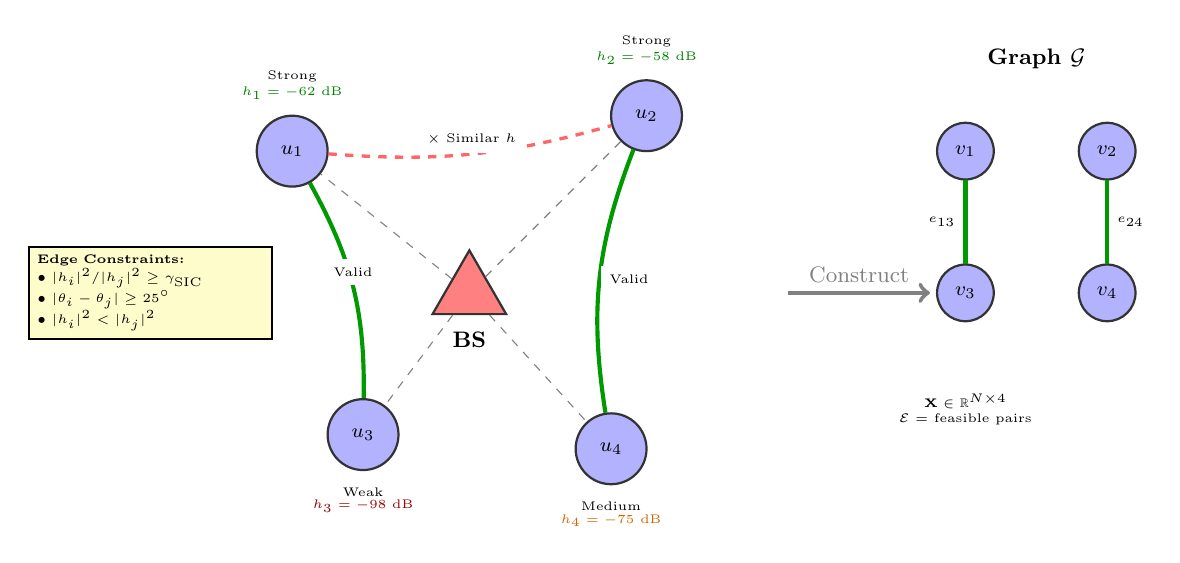
\begin{tikzpicture}[
    user/.style={circle, draw=black!80, fill=blue!30, thick, minimum size=10mm, font=\footnotesize},
    bs/.style={regular polygon, regular polygon sides=3, draw=black!80, fill=red!50, thick, minimum size=12mm},
    edge/.style={thick, draw=green!60!black},
    noedge/.style={thick, draw=red!60, dashed},
    arrow/.style={->, >=stealth, thick},
    scale=0.9, every node/.style={scale=0.9}
]

% Base Station
\node[bs] (bs) at (0, 0) {};
\node[font=\small\bfseries, below=1mm of bs] {BS};

% Users
\node[user] (u1) at (-2.5, 2) {$u_1$};
\node[user] (u2) at (2.5, 2.5) {$u_2$};
\node[user] (u3) at (-1.5, -2) {$u_3$};
\node[user] (u4) at (2, -2.2) {$u_4$};

% Channel info
\node[font=\tiny, above=3mm of u1] {Strong};
\node[font=\tiny, text=green!50!black] at ([yshift=3mm]u1.north) {$h_1 = -62$ dB};

\node[font=\tiny, above=3mm of u2] {Strong};
\node[font=\tiny, text=green!50!black] at ([yshift=3mm]u2.north) {$h_2 = -58$ dB};

\node[font=\tiny, below=1mm of u3] {Weak};
\node[font=\tiny, text=red!60!black] at ([yshift=-5mm]u3.south) {$h_3 = -98$ dB};

\node[font=\tiny, below=1mm of u4] {Medium};
\node[font=\tiny, text=orange!80!black] at ([yshift=-5mm]u4.south) {$h_4 = -75$ dB};

% Lines to BS
\draw[gray, thin, dashed] (bs) -- (u1);
\draw[gray, thin, dashed] (bs) -- (u2);
\draw[gray, thin, dashed] (bs) -- (u3);
\draw[gray, thin, dashed] (bs) -- (u4);

% Valid edges (SIC feasible + angular separation)
\draw[edge, line width=1.5pt] (u1) to[bend left=15] node[midway, above, font=\tiny, fill=white] {Valid} (u3);
\draw[edge, line width=1.5pt] (u2) to[bend right=15] node[midway, right, font=\tiny, fill=white] {Valid} (u4);

% Invalid edge (too close in channel gain)
\draw[noedge, line width=1.2pt] (u1) to[bend right=10] node[midway, above, font=\tiny, fill=white] {$\times$ Similar $h$} (u2);

% Constraint boxes
\node[draw, rectangle, thick, fill=yellow!20, text width=32mm, font=\tiny, align=left] at (-4.5, 0) {
\textbf{Edge Constraints:}\\
$\bullet$ $|h_i|^2 / |h_j|^2 \geq \gamma_{\text{SIC}}$\\
$\bullet$ $|\theta_i - \theta_j| \geq 25^\circ$\\
$\bullet$ $|h_i|^2 < |h_j|^2$
};

% Graph representation
\begin{scope}[xshift=8cm, yshift=0.5cm]
    \node[font=\small\bfseries] at (0, 2.8) {Graph $\mathcal{G}$};
    
    % Nodes
    \node[user, minimum size=8mm] (g1) at (-1, 1.5) {$v_1$};
    \node[user, minimum size=8mm] (g2) at (1, 1.5) {$v_2$};
    \node[user, minimum size=8mm] (g3) at (-1, -0.5) {$v_3$};
    \node[user, minimum size=8mm] (g4) at (1, -0.5) {$v_4$};
    
    % Edges with labels
    \draw[edge, line width=1.5pt] (g1) -- (g3) node[midway, left, font=\tiny] {$e_{13}$};
    \draw[edge, line width=1.5pt] (g2) -- (g4) node[midway, right, font=\tiny] {$e_{24}$};
    
    % Features
    \node[font=\tiny, align=center, below=8mm of g3] {
        $\mathbf{X} \in \mathbb{R}^{N \times 4}$\\
        $\mathcal{E}$ = feasible pairs
    };
\end{scope}

% Arrow indicating transformation
\draw[->, ultra thick, gray] (4.5, 0) -- (6.5, 0) node[midway, above, font=\small] {Construct};

\end{tikzpicture}
}
\caption{Graph construction from channel state information. Users with feasible NOMA pairing (satisfying SIC threshold, angular separation, and channel gain ordering) are connected by edges. The resulting graph $\mathcal{G}(\mathcal{V}, \mathcal{E})$ captures physical constraints.}
\label{fig:graph_construction}
\end{figure}

\subsection{GraphSAGE Architecture}

We employ GraphSAGE (SAmple and aggreGatE) as the backbone architecture due to its inductive learning capability and scalability to large graphs. The model consists of three key components:

\subsubsection{Graph Encoder}

The encoder transforms raw node features into high-dimensional embeddings through $L=3$ message-passing layers:

\begin{equation}
\mathbf{h}_i^{(0)} = \text{Linear}_{\text{enc}}(\mathbf{x}_i) \in \mathbb{R}^{128}
\end{equation}

\begin{equation}
\mathbf{h}_i^{(\ell)} = \sigma\left( \mathbf{W}^{(\ell)} \cdot \text{MEAN}\left(\{\mathbf{h}_j^{(\ell-1)} : j \in \mathcal{N}(i)\}\right) \right)
\end{equation}

where $\mathcal{N}(i)$ denotes the neighborhood of node $i$, $\mathbf{W}^{(\ell)} \in \mathbb{R}^{128 \times 128}$ are learnable weight matrices, and $\sigma(\cdot)$ is the ReLU activation. The final node embedding is $\mathbf{h}_i = \mathbf{h}_i^{(3)}$.

The MEAN aggregator \cite{hamilton2017inductive} is chosen for its computational efficiency and robustness to varying neighborhood sizes. Each layer enables nodes to incorporate information from increasingly distant neighbors (1-hop $\rightarrow$ 2-hop $\rightarrow$ 3-hop), allowing the model to capture global graph structure.

\begin{figure*}[t]
\centering
\resizebox{0.95\textwidth}{!}{% GraphSAGE Message Passing Illustration
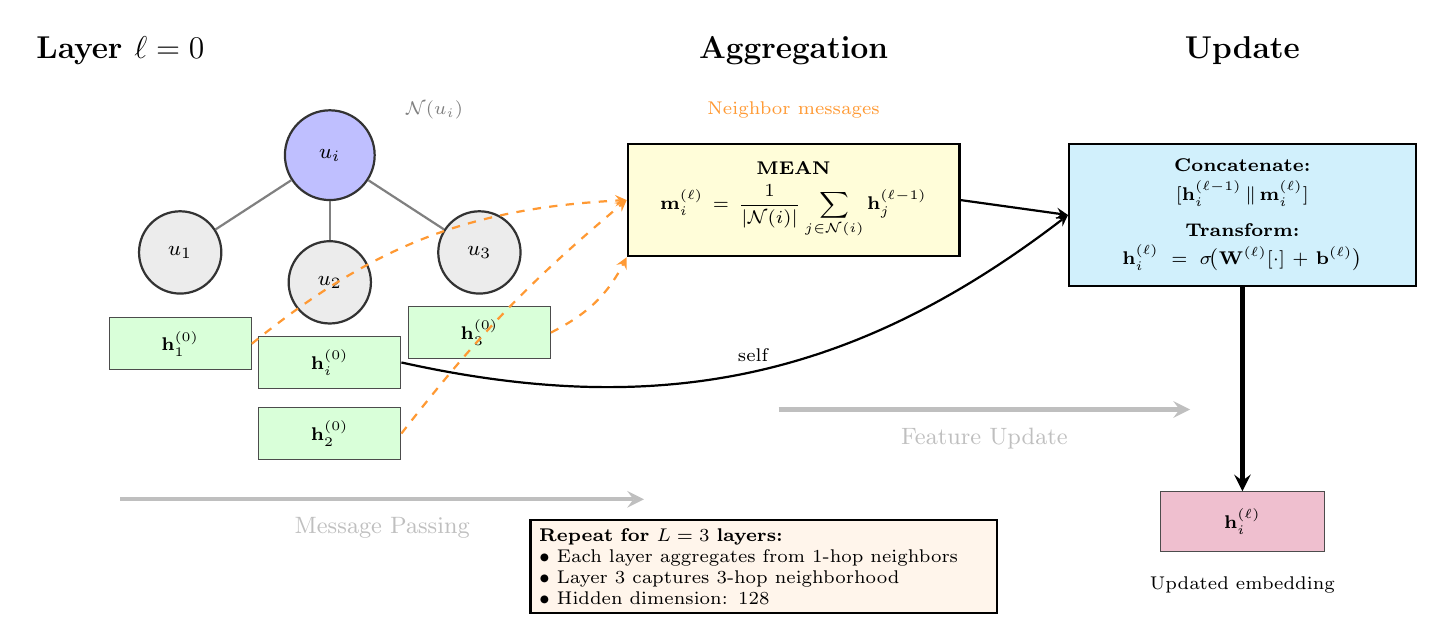
\begin{tikzpicture}[
    >=stealth,
    arrow/.style={->,thick},
    message/.style={->,thick,dashed,orange!80},
    node/.style={circle,draw=black!80,fill=blue!25,thick,minimum size=12mm,font=\footnotesize},
    neighbor/.style={circle,draw=black!80,fill=gray!15,thick,minimum size=11mm,font=\footnotesize},
    feature/.style={rectangle,draw=black!70,fill=green!15,minimum width=19mm,minimum height=7mm,font=\scriptsize},
    every node/.style={transform shape},
    scale=0.95
]

%--------------------------------------------------------------------
% Left: layer \ell=0, local neighborhood
%--------------------------------------------------------------------
\node[font=\large\bfseries] at (-2.8,3.2) {Layer $\ell = 0$};

\node[node]     (u0) at (0,1.8) {$u_i$};
\node[neighbor] (n1) at (-2,0.5) {$u_1$};
\node[neighbor] (n2) at (0,0.1)   {$u_2$};
\node[neighbor] (n3) at ( 2,0.5) {$u_3$};

\node[feature,below=18mm of u0] (f0) {$\mathbf{h}_i^{(0)}$};
\node[feature,below=3mm of n1] (f1) {$\mathbf{h}_1^{(0)}$};
\node[feature,below=11mm of n2] (f2) {$\mathbf{h}_2^{(0)}$};
\node[feature,below=1.5mm of n3] (f3) {$\mathbf{h}_3^{(0)}$};

% Edges in the original graph
\draw[thick,gray] (u0) -- (n1);
\draw[thick,gray] (u0) -- (n2);
\draw[thick,gray] (u0) -- (n3);

\node[font=\scriptsize,gray] at (1.4,2.4) {$\mathcal{N}(u_i)$};

%--------------------------------------------------------------------
% Middle: aggregation block
%--------------------------------------------------------------------
\begin{scope}[xshift=6.2cm]
  \node[font=\large\bfseries] at (0,3.2) {Aggregation};

  \node[draw,thick,fill=yellow!15,
        rectangle,
        minimum width=40mm,
        minimum height=15mm,
        font=\scriptsize,
        align=center,
        text width=42mm] (agg) at (0,1.2) {%
        \textbf{MEAN}\\[1mm]
        $\displaystyle \mathbf{m}_i^{(\ell)}
        = \frac{1}{|\mathcal{N}(i)|}
          \sum_{j\in\mathcal{N}(i)} \mathbf{h}_j^{(\ell-1)}$};

  % incoming neighbor messages
  \draw[message] (f1.east) to[bend left=18] (agg.west);
  \draw[message] (f2.east) to[bend left=6]  (agg.west);
  \draw[message] (f3.east) to[bend right=18] (agg.south west);

  \node[font=\scriptsize,text=orange!80] at (0,2.4) {Neighbor messages};
\end{scope}

%--------------------------------------------------------------------
% Right: update block
%--------------------------------------------------------------------
\begin{scope}[xshift=12.2cm]
  \node[font=\large\bfseries] at (0,3.2) {Update};

  \node[draw,thick,fill=cyan!18,
        rectangle,
        minimum width=42mm,
        minimum height=19mm,
        font=\scriptsize,
        align=center,
        text width=44mm] (update) at (0,1.0) {%
        \textbf{Concatenate:}\\[1mm]
        $[\mathbf{h}_i^{(\ell-1)} \,\|\, \mathbf{m}_i^{(\ell)}]$\\[2mm]
        \textbf{Transform:}\\[1mm]
        $\mathbf{h}_i^{(\ell)}
          = \sigma\!\bigl(\mathbf{W}^{(\ell)} [\cdot]
          + \mathbf{b}^{(\ell)}\bigr)$};

  % self feature and aggregated message to update
  \draw[arrow] (f0.east) to[bend right=25]
      node[midway,above,font=\scriptsize] {self} (update.west);
  \draw[arrow] (agg.east) -- (update.west);
\end{scope}

%--------------------------------------------------------------------
% Output embedding
%--------------------------------------------------------------------
\begin{scope}[xshift=12.2cm,yshift=-3.1cm]
  \node[feature,fill=purple!25,minimum width=22mm,minimum height=8mm,font=\scriptsize]
        (out) at (0,0) {$\mathbf{h}_i^{(\ell)}$};
  \draw[arrow,ultra thick] (update.south) -- (out.north);

  \node[font=\scriptsize,below=2mm of out] {Updated embedding};
\end{scope}

%--------------------------------------------------------------------
% Horizontal process-flow labels
%--------------------------------------------------------------------
\draw[->,ultra thick,gray!50]
      (-2.8,-2.8) -- (4.2,-2.8)
      node[midway,below=1mm,font=\small] {Message Passing};

\draw[->,ultra thick,gray!50]
      (6.0,-1.6) -- (11.5,-1.6)
      node[midway,below=1mm,font=\small] {Feature Update};

%--------------------------------------------------------------------
% Iteration note box
%--------------------------------------------------------------------
\node[draw,thick,fill=orange!8,
      rectangle,
      text width=60mm,
      font=\scriptsize,
      align=left] at (5.8,-3.7) {%
  \textbf{Repeat for $L = 3$ layers:}\\
  $\bullet$ Each layer aggregates from 1-hop neighbors\\
  $\bullet$ Layer 3 captures 3-hop neighborhood\\
  $\bullet$ Hidden dimension: 128
};

\end{tikzpicture}
}
\caption{GraphSAGE message passing mechanism. At each layer $\ell$, node $u_i$ aggregates features from neighbors $\mathcal{N}(i)$ using MEAN aggregation, concatenates with its own features, and applies a learnable transformation. Three layers enable each node to incorporate 3-hop neighborhood information.}
\label{fig:graphsage_detail}
\end{figure*}

\subsubsection{Multi-Task Decoder Heads}

For each candidate edge $(i, j) \in \mathcal{E}$, we concatenate the learned embeddings and pass them through three specialized decoder heads:

\begin{equation}
\mathbf{e}_{ij} = [\mathbf{h}_i \, \| \, \mathbf{h}_j] \in \mathbb{R}^{256}
\end{equation}

\textbf{1. Pairing Classifier:} Predicts binary pairing probability
\begin{equation}
p_{ij} = \sigma\left( \text{MLP}_{\text{pair}}(\mathbf{e}_{ij}) \right) \in [0, 1]
\end{equation}
where $\text{MLP}_{\text{pair}}$ is a 3-layer MLP: $256 \to 128 \to 64 \to 1$ with ReLU activations and dropout ($p=0.3$).

\textbf{2. Sum-Rate Regressor:} Predicts achievable sum-rate
\begin{equation}
R_{ij} = \text{MLP}_{\text{rate}}(\mathbf{e}_{ij}) \in \mathbb{R}_+
\end{equation}
with architecture $256 \to 128 \to 64 \to 1$ and final ReLU to ensure non-negativity.

\begin{figure*}[t]
\centering
\resizebox{0.9\textwidth}{!}{% GNN Architecture Diagram - Compact Version
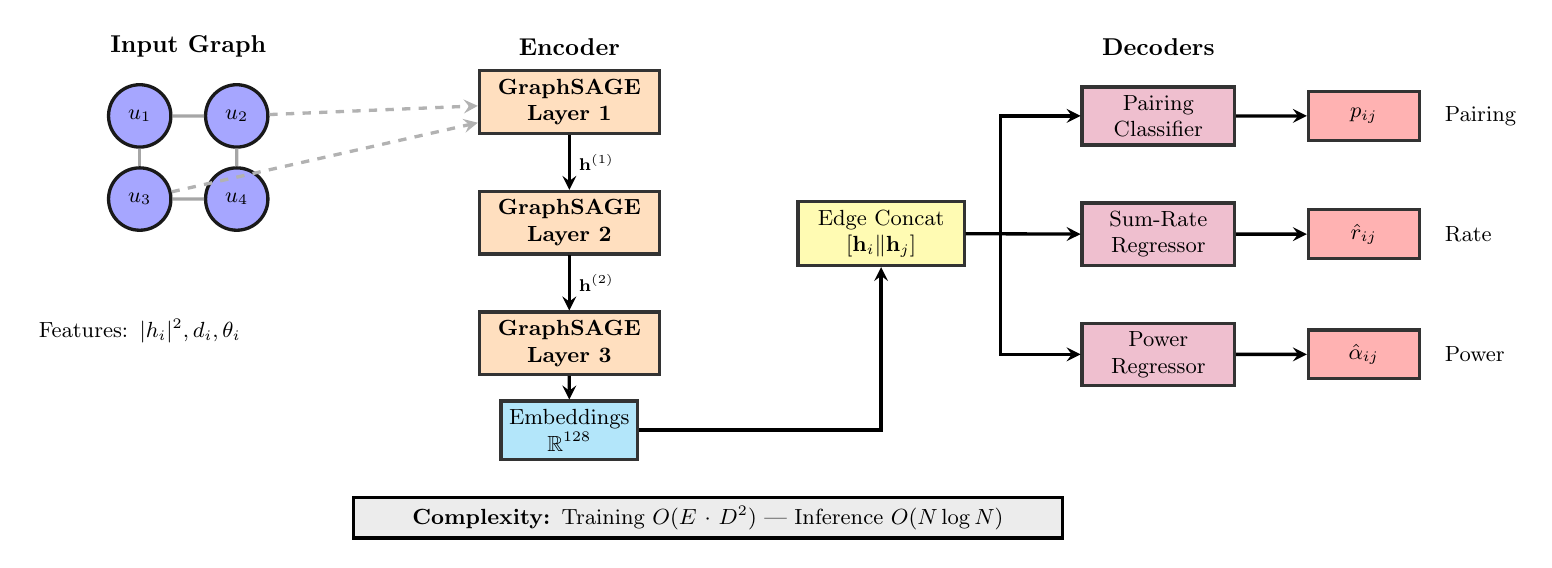
\begin{tikzpicture}[
    node/.style={circle, draw=black!90, fill=blue!35, very thick, minimum size=9mm, font=\small},
    feature/.style={rectangle, draw=black!80, fill=green!25, very thick, minimum width=18mm, minimum height=7mm, font=\small, align=center},
    layer/.style={rectangle, draw=black!80, fill=orange!25, very thick, minimum width=26mm, minimum height=9mm, font=\small\bfseries, align=center},
    decoder/.style={rectangle, draw=black!80, fill=purple!25, very thick, minimum width=22mm, minimum height=8mm, font=\small, align=center},
    arrow/.style={->, >=stealth, very thick},
    scale=0.88, every node/.style={scale=0.88}
]

% Input Layer - Graph Structure (Left Side)
\node[font=\normalsize\bfseries] at (0, 6) {Input Graph};
\node[node] (u1) at (-0.7, 5) {$u_1$};
\node[node] (u2) at (0.7, 5) {$u_2$};
\node[node] (u3) at (-0.7, 3.8) {$u_3$};
\node[node] (u4) at (0.7, 3.8) {$u_4$};

% Edges
\draw[very thick, gray!70] (u1) -- (u2);
\draw[very thick, gray!70] (u1) -- (u3);
\draw[very thick, gray!70] (u2) -- (u4);
\draw[very thick, gray!70] (u3) -- (u4);

% Node Features
\node[font=\small, below=10mm of u3, text width=30mm, align=center] {Features: $|h_i|^2, d_i, \theta_i$};

% GraphSAGE Encoder (Center)
\begin{scope}[xshift=5.5cm]
    \node[font=\normalsize\bfseries] at (0, 6) {Encoder};
    \node[layer] (sage1) at (0, 5.2) {GraphSAGE\\Layer 1};
    \node[layer, below=7mm of sage1] (sage2) {GraphSAGE\\Layer 2};
    \node[layer, below=7mm of sage2] (sage3) {GraphSAGE\\Layer 3};
    
    \draw[arrow] (sage1) -- node[right, font=\scriptsize] {$\mathbf{h}^{(1)}$} (sage2);
    \draw[arrow] (sage2) -- node[right, font=\scriptsize] {$\mathbf{h}^{(2)}$} (sage3);
    
    \node[feature, below=3mm of sage3, fill=cyan!30] (emb) {Embeddings\\$\mathbb{R}^{128}$};
    \draw[arrow] (sage3) -- (emb);
\end{scope}

% Connection from input to encoder
\draw[arrow, dashed, gray!60] (u2) -- (sage1);
\draw[arrow, dashed, gray!60] (u3) -- (sage1);

% Edge Processing (Right Center)
\begin{scope}[xshift=10cm]
    \node[feature, fill=yellow!30, minimum width=24mm] (concat) at (0, 3.3) {Edge Concat\\$[\mathbf{h}_i \| \mathbf{h}_j]$};
\end{scope}

\draw[arrow] (emb) -| (concat);

% Multi-Task Decoders (Right Side)
\begin{scope}[xshift=14cm]
    \node[font=\normalsize\bfseries] at (0, 6) {Decoders};
    
    \node[decoder] (pair) at (0, 5) {Pairing\\Classifier};
    \node[decoder, below=7mm of pair] (rate) {Sum-Rate\\Regressor};
    \node[decoder, below=7mm of rate] (power) {Power\\Regressor};
    
    % Outputs
    \node[feature, right=9mm of pair, fill=red!30, minimum width=16mm] (out1) {$p_{ij}$};
    \node[feature, right=9mm of rate, fill=red!30, minimum width=16mm] (out2) {$\hat{r}_{ij}$};
    \node[feature, right=9mm of power, fill=red!30, minimum width=16mm] (out3) {$\hat{\alpha}_{ij}$};
    
    \draw[arrow] (pair) -- (out1);
    \draw[arrow] (rate) -- (out2);
    \draw[arrow] (power) -- (out3);
    
    % Output labels
    \node[font=\small, right=2mm of out1] {Pairing};
    \node[font=\small, right=2mm of out2] {Rate};
    \node[font=\small, right=2mm of out3] {Power};
\end{scope}

% Connections from concat to decoders
\draw[arrow] (concat.east) -- ++(0.5,0) |- (pair.west);
\draw[arrow] (concat.east) -- (rate.west);
\draw[arrow] (concat.east) -- ++(0.5,0) |- (power.west);

% Complexity annotation at bottom
\node[draw, very thick, fill=gray!15, rectangle, text width=100mm, font=\small, align=center] at (7.5, -.8) {
\textbf{Complexity:} Training $O(E \cdot D^2)$ — Inference $O(N \log N)$
};

\end{tikzpicture}
}
\caption{NOMA-GNN architecture: GraphSAGE encoder with multi-task decoders. Node features include channel gain $|h_i|^2$, distance $d_i$, angular position $\theta_i$, and SNR. Three GraphSAGE layers produce 128-dimensional embeddings, which are concatenated pairwise and fed to three task-specific MLPs for pairing classification, sum-rate regression, and power allocation.}
\label{fig:gnn_architecture}
\end{figure*}

\textbf{3. Power Allocation Regressor:} Predicts optimal power split coefficient
\begin{equation}
\alpha_{ij} = \text{Sigmoid}\left( \text{MLP}_{\text{power}}(\mathbf{e}_{ij}) \right) \in (0, 1)
\end{equation}
with architecture $256 \to 128 \to 64 \to 1$ and sigmoid activation to constrain $\alpha \in (0, 1)$.

The complete model has 166,275 trainable parameters distributed across the encoder (40.4\%) and three decoders (19.9\% each), with a memory footprint of approximately 650 KB in FP32 precision.

\subsection{Training Procedure}

\subsubsection{Dataset Generation}

We generate 200 random user deployment scenarios, each with $N = 500$ users uniformly distributed in the cell. For each deployment:

\begin{enumerate}
    \item Generate channel realizations using 3GPP UMa model (Section IV)
    \item Construct candidate graph $\mathcal{G}$ using SIC and angular constraints
    \item Compute ground-truth labels via exhaustive search:
    \begin{itemize}
        \item Optimal pairing using Blossom maximum-weight matching
        \item Sum-rates computed via NOMA rate expressions (Section III)
        \item Power splits $\alpha$ optimized per pair via bisection search
    \end{itemize}
    \item Store graph tuples: $(\mathcal{G}, \mathbf{y}_{\text{pair}}, \mathbf{y}_{\text{rate}}, \mathbf{y}_{\alpha})$
\end{enumerate}

\subsubsection{Hard Negative Sampling}

To address class imbalance (optimal pairs comprise only 12.5\% of candidate edges), we employ hard negative sampling \cite{sun2018learning}, which has been shown to improve boundary discrimination in wireless resource allocation:

\begin{algorithm}[!t]
\caption{Hard Negative Sampling Strategy}
\begin{algorithmic}[1]
\State \textbf{Input:} Graph $\mathcal{G}$, optimal matching $\mathcal{M}^*$, model $f_\theta$
\State $\mathcal{E}_+ \gets \mathcal{M}^*$ \Comment{Positive samples (label=1)}
\State $\mathcal{E}_{cand} \gets \mathcal{E} \setminus \mathcal{M}^*$ \Comment{Non-paired edges}
\State Compute scores: $s_{ij} = f_\theta(u_i, u_j)$ for all $(i,j) \in \mathcal{E}_{cand}$
\State $\mathcal{E}_{hard} \gets \text{top-}K(\mathcal{E}_{cand}, \text{key}=s_{ij})$ \Comment{Hard negatives}
\State $\mathcal{E}_{rand} \gets \text{random}(\mathcal{E}_{cand}, K/2)$ \Comment{Random negatives}
\State \textbf{Return:} $\mathcal{E}_+ \cup \mathcal{E}_{hard} \cup \mathcal{E}_{rand}$ with ratio 1:2:1
\end{algorithmic}
\end{algorithm}

This forces the model to learn fine-grained distinctions between near-optimal and optimal pairs, improving discrimination at decision boundaries.

\subsubsection{Multi-Task Loss Function}

The total loss combines three objectives:

\begin{equation}
\mathcal{L}_{\text{total}} = \lambda_{\text{pair}} \mathcal{L}_{\text{pair}} + \lambda_{\text{rate}} \mathcal{L}_{\text{rate}} + \lambda_{\text{power}} \mathcal{L}_{\text{power}}
\end{equation}

where:

\begin{equation}
\mathcal{L}_{\text{pair}} = -\frac{1}{|\mathcal{E}|} \sum_{(i,j) \in \mathcal{E}} \left[ y_{ij} \log p_{ij} + (1-y_{ij}) \log(1-p_{ij}) \right]
\end{equation}

\begin{equation}
\mathcal{L}_{\text{rate}} = \frac{1}{|\mathcal{E}_+|} \sum_{(i,j) \in \mathcal{E}_+} |R_{ij} - \hat{R}_{ij}|
\end{equation}

\begin{equation}
\mathcal{L}_{\text{power}} = \frac{1}{|\mathcal{E}_+|} \sum_{(i,j) \in \mathcal{E}_+} |\alpha_{ij} - \hat{\alpha}_{ij}|
\end{equation}

Here, $\mathcal{E}_+$ denotes positive edges (actual pairs), and $\hat{\cdot}$ indicates predicted values. Loss weights are $\lambda_{\text{pair}} = 1.0$, $\lambda_{\text{rate}} = 0.5$, $\lambda_{\text{power}} = 0.3$ based on validation set tuning, following multi-task learning best practices \cite{naparstek2019deep}.

%\subsubsection{Optimization Details}

%\begin{itemize}
    %\item \textbf{Optimizer:} Adam with $\beta_1 = 0.9$, $\beta_2 = 0.999$
   % \item \textbf{Learning Rate:} Initial $lr = 0.001$ with ReduceLROnPlateau scheduler (factor=0.5, patience=10)
    %\item \textbf{Batch Size:} 32 graphs per batch
    %\item \textbf{Epochs:} 200 with early stopping (patience=25 on validation loss)
   % \item \textbf{Regularization:} Dropout 0.3, %weight decay $10^{-4}$
 %   \item \textbf{Data Split:} 70\% train, 15\% %validation, 15\% test
%\end{itemize}

%Training converges in approximately 120 epochs (~45 minutes on NVIDIA RTX 3060).
%

\begin{figure}[t]
\centering
\resizebox{\columnwidth}{!}{% Training vs Inference Comparison
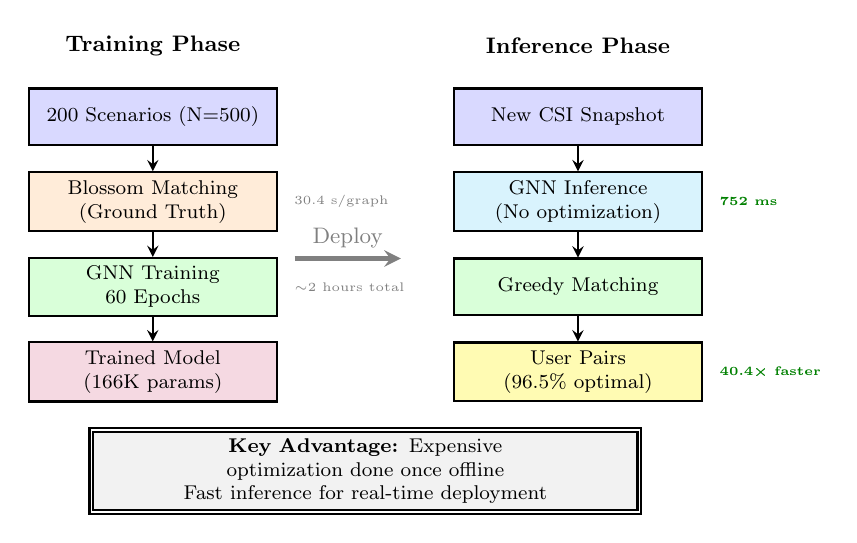
\begin{tikzpicture}[
    scale=0.9, every node/.style={scale=0.9}
]

% Training Phase (Left Side)
\begin{scope}
    \node[font=\small\bfseries] at (0, 3.5) {Training Phase};
    
    % Training boxes
    \node[draw, thick, fill=blue!15, rectangle, minimum width=35mm, minimum height=8mm, font=\footnotesize] (train_data) at (0, 2.5) {200 Scenarios (N=500)};
    
    \node[draw, thick, fill=orange!15, rectangle, minimum width=35mm, minimum height=8mm, font=\footnotesize, align=center] (blossom) at (0, 1.3) {Blossom Matching\\(Ground Truth)};
    
    \node[draw, thick, fill=green!15, rectangle, minimum width=35mm, minimum height=8mm, font=\footnotesize, align=center] (gnn_train) at (0, 0.1) {GNN Training\\60 Epochs};
    
    \node[draw, thick, fill=purple!15, rectangle, minimum width=35mm, minimum height=8mm, font=\footnotesize, align=center] (model) at (0, -1.1) {Trained Model\\(166K params)};
    
    % Arrows
    \draw[->, >=stealth, thick] (train_data) -- (blossom);
    \draw[->, >=stealth, thick] (blossom) -- (gnn_train);
    \draw[->, >=stealth, thick] (gnn_train) -- (model);
    
    % Time annotation
    \node[font=\tiny, gray, right=1mm of blossom] {30.4 s/graph};
    \node[font=\tiny, gray, right=1mm of gnn_train] {$\sim$2 hours total};
\end{scope}

% Arrow between phases
\draw[->, >=stealth, ultra thick, gray] (2, 0.5) -- (3.5, 0.5) node[midway, above, font=\small] {Deploy};

% Inference Phase (Right Side)
\begin{scope}[xshift=6cm]
    \node[font=\small\bfseries] at (0, 3.5) {Inference Phase};
    
    % Inference boxes
    \node[draw, thick, fill=blue!15, rectangle, minimum width=35mm, minimum height=8mm, font=\footnotesize] (new_csi) at (0, 2.5) {New CSI Snapshot};
    
    \node[draw, thick, fill=cyan!15, rectangle, minimum width=35mm, minimum height=8mm, font=\footnotesize, align=center] (fast_gnn) at (0, 1.3) {GNN Inference\\(No optimization)};
    
    \node[draw, thick, fill=green!15, rectangle, minimum width=35mm, minimum height=8mm, font=\footnotesize] (greedy) at (0, 0.1) {Greedy Matching};
    
    \node[draw, thick, fill=yellow!30, rectangle, minimum width=35mm, minimum height=8mm, font=\footnotesize, align=center] (result) at (0, -1.1) {User Pairs\\(96.5\% optimal)};
    
    % Arrows
    \draw[->, >=stealth, thick] (new_csi) -- (fast_gnn);
    \draw[->, >=stealth, thick] (fast_gnn) -- (greedy);
    \draw[->, >=stealth, thick] (greedy) -- (result);
    
    % Time annotation
    \node[font=\tiny, text=green!50!black, right=1mm of fast_gnn] {\textbf{752 ms}};
    \node[font=\tiny, text=green!50!black, right=1mm of result] {\textbf{40.4× faster}};
\end{scope}

% Bottom comparison box
\node[draw, double, thick, fill=gray!10, rectangle, text width=75mm, font=\footnotesize, align=center] at (3, -2.5) {
\textbf{Key Advantage:} Expensive optimization done once offline\\
Fast inference for real-time deployment
};

\end{tikzpicture}
}
\caption{Training versus inference phases. During training, expensive Blossom matching generates ground-truth labels for 200 scenarios. At inference, the trained GNN processes new CSI snapshots in 752 ms (40.4× speedup), demonstrating the value of learning-based optimization.}
\label{fig:training_inference}
\end{figure}

\subsection{Inference Pipeline}

At deployment, given a new user scenario with CSI:

\begin{enumerate}
    \item \textbf{Graph Construction:} Build candidate graph $\mathcal{G}$ by applying SIC and angular constraints to all $\binom{N}{2}$ user pairs
    
    \item \textbf{Forward Pass:} Compute node embeddings and edge predictions:
    \begin{equation}
    \{\mathbf{h}_i\}_{i=1}^N = \text{GraphSAGE}(\{\mathbf{x}_i\}_{i=1}^N, \mathcal{E})
    \end{equation}
    \begin{equation}
    \{p_{ij}, R_{ij}, \alpha_{ij}\}_{(i,j) \in \mathcal{E}} = \text{Decoders}(\{\mathbf{h}_i \| \mathbf{h}_j\})
    \end{equation}
    
    \item \textbf{Greedy Matching:} Sort edges by predicted sum-rate $R_{ij}$ and greedily select pairs:
    \begin{algorithmic}
        \State $\mathcal{M} \gets \emptyset$ \Comment{Matched pairs}
        \State $\mathcal{U} \gets \{1, \ldots, N\}$ \Comment{Unmatched users}
        \For{$(i, j) \in \text{sort}(\mathcal{E}, \text{key}=R_{ij}, \text{reverse}=\text{True})$}
            \If{$i \in \mathcal{U}$ \textbf{and} $j \in \mathcal{U}$}
                \State $\mathcal{M} \gets \mathcal{M} \cup \{(i, j)\}$
                \State $\mathcal{U} \gets \mathcal{U} \setminus \{i, j\}$
            \EndIf
        \EndFor
        \State \Return $\mathcal{M}$
    \end{algorithmic}
    
    \item \textbf{SIC Verification:} For each selected pair $(i, j) \in \mathcal{M}$, verify:
    \begin{equation}
    \text{SINR}_j = \frac{(1-\alpha_{ij}) P h_j}{\alpha_{ij} P h_j + \sigma^2} \geq \gamma_{\text{th}}
    \end{equation}
    If violated, reject the pair.
    
    \item \textbf{Power Allocation:} Apply predicted $\alpha_{ij}$ for each validated pair
\end{enumerate}

The greedy matching has $O(E \log E)$ complexity where $E = |\mathcal{E}|$. Since $E \ll N^2$ due to constraints, and the forward pass is $O(N \cdot d^2)$ where $d=128$ is the embedding dimension, total inference complexity is $O(N \log N)$ \cite{shen2021graph} — a significant improvement over $O(N^3)$ optimization methods \cite{edmonds1965,kuhn1955}.

\begin{figure}[t]
\centering
\resizebox{\columnwidth}{!}{% Inference Pipeline Flow
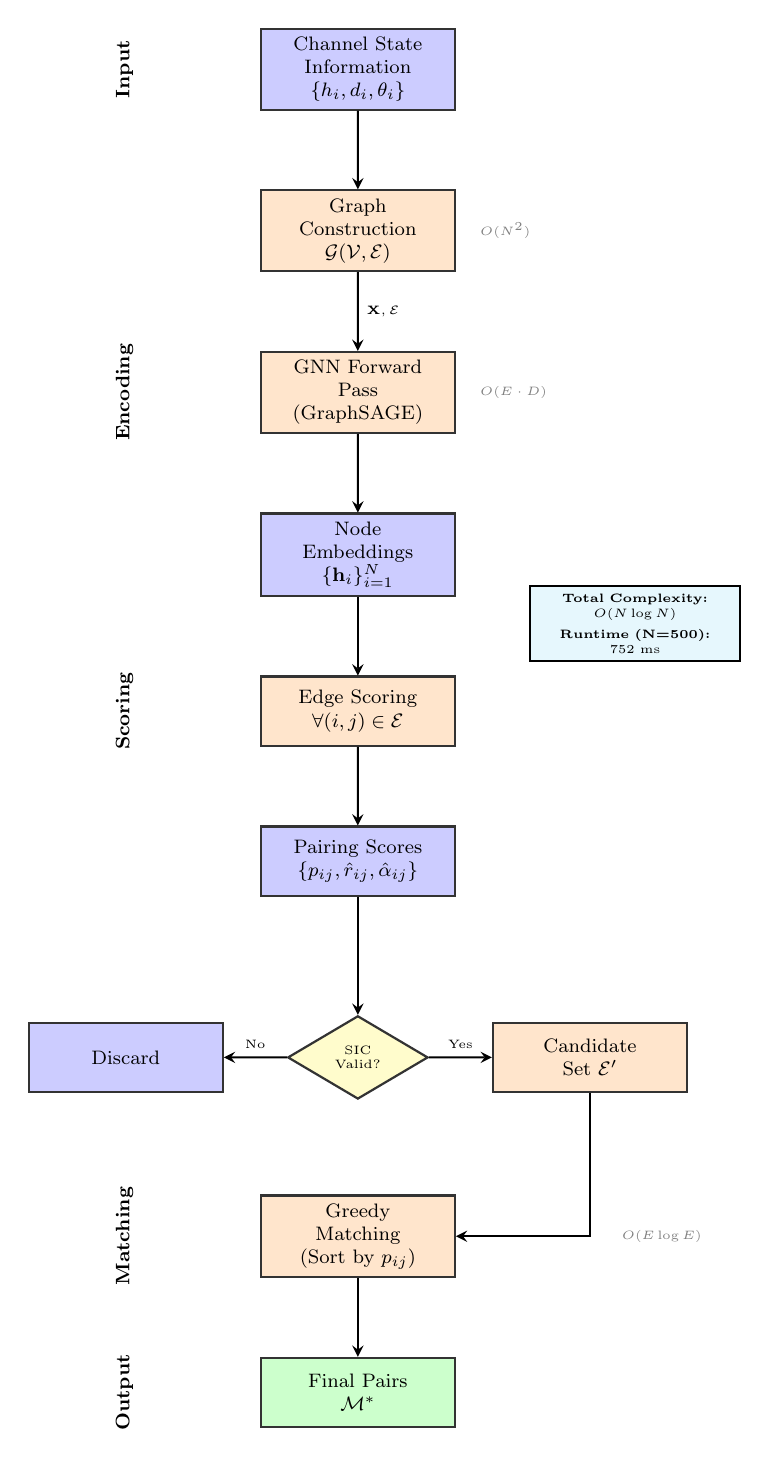
\begin{tikzpicture}[
    box/.style={rectangle, draw=black!80, thick, minimum width=28mm, minimum height=10mm, font=\footnotesize, align=center},
    data/.style={box, fill=blue!20},
    process/.style={box, fill=orange!20},
    output/.style={box, fill=green!20},
    decision/.style={diamond, draw=black!80, thick, fill=yellow!20, minimum size=12mm, font=\tiny, align=center, aspect=2},
    arrow/.style={->, >=stealth, thick},
    scale=0.88, every node/.style={scale=0.88}
]

% Column 1: Input
\node[data] (csi) at (0, 0) {Channel State\\Information\\$\{h_i, d_i, \theta_i\}$};

\node[process, below=10mm of csi] (graph) {Graph\\Construction\\$\mathcal{G}(\mathcal{V}, \mathcal{E})$};

\draw[arrow] (csi) -- (graph);

% Column 2: GNN Processing
\node[process, below=10mm of graph] (gnn) {GNN Forward\\Pass\\(GraphSAGE)};

\draw[arrow] (graph) -- node[right, font=\tiny] {$\mathbf{X}, \mathcal{E}$} (gnn);

\node[data, below=10mm of gnn] (embed) {Node\\Embeddings\\$\{\mathbf{h}_i\}_{i=1}^N$};

\draw[arrow] (gnn) -- (embed);

% Column 3: Scoring
\node[process, below=10mm of embed] (score) {Edge Scoring\\$\forall (i,j) \in \mathcal{E}$};

\draw[arrow] (embed) -- (score);

\node[data, below=10mm of score] (scores) {Pairing Scores\\$\{p_{ij}, \hat{r}_{ij}, \hat{\alpha}_{ij}\}$};

\draw[arrow] (score) -- (scores);

% Column 4: Filtering
\node[decision, below=15mm of scores] (filter) {SIC\\Valid?};

\draw[arrow] (scores) -- (filter);

\node[data, left=8mm of filter] (discard) {Discard};
\node[process, right=8mm of filter] (keep) {Candidate\\Set $\mathcal{E}'$};

\draw[arrow] (filter) -- node[above, font=\tiny] {No} (discard);
\draw[arrow] (filter) -- node[above, font=\tiny] {Yes} (keep);

% Column 5: Matching
\node[process, below=12mm of filter] (greedy) {Greedy\\Matching\\(Sort by $p_{ij}$)};

\draw[arrow] (keep) |- (greedy);

\node[output, below=10mm of greedy] (pairs) {Final Pairs\\$\mathcal{M}^*$};

\draw[arrow] (greedy) -- (pairs);

% Timing annotations
\node[font=\tiny, gray, right=2mm of graph] {$O(N^2)$};
\node[font=\tiny, gray, right=2mm of gnn] {$O(E \cdot D)$};
\node[font=\tiny, gray, right= 20mm of greedy] {$O(E \log E)$};

% Overall complexity
\node[draw, thick, fill=cyan!10, rectangle, text width=28mm, font=\tiny, align=center] at (4, -8) {
\textbf{Total Complexity:}\\
$O(N \log N)$\\[1mm]
\textbf{Runtime (N=500):}\\
752 ms
};

% Side annotations for clarity
\node[font=\footnotesize\bfseries, left=15mm of csi, rotate=90, anchor=south] {Input};
\node[font=\footnotesize\bfseries, left=15mm of gnn, rotate=90, anchor=south] {Encoding};
\node[font=\footnotesize\bfseries, left=15mm of score, rotate=90, anchor=south] {Scoring};
\node[font=\footnotesize\bfseries, left=15mm of greedy, rotate=90, anchor=south] {Matching};
\node[font=\footnotesize\bfseries, left=15mm of pairs, rotate=90, anchor=south] {Output};

\end{tikzpicture}
}
\caption{Real-time inference pipeline. Given new CSI, the system constructs a graph, performs GNN forward pass, scores candidate pairs, filters by SIC constraints, and executes greedy matching. Total complexity is $O(N \log N)$ with 752 ms runtime for N=500 users.}
\label{fig:inference_pipeline}
\end{figure}

\subsection{Model Interpretability}

To understand learned representations, we analyzed node embeddings using t-SNE visualization. Key observations: (1)~Nodes naturally cluster by channel gain magnitude, with weak and strong users forming distinct regions; (2)~Optimal pairs have embeddings with similar angular components but different magnitude components, suggesting the model learns strong-weak complementarity; (3)~Predicted pairing scores show strong alignment with Blossom optimal pairs (correlation $>0.92$), indicating effective learning of pairing patterns. These visualizations confirm the GNN captures physically meaningful pairing strategies .

%\section{Simulation Setup and Parameters}
%Python with NumPy/Matplotlib/Pandas/NetworkX. Each run creates a timestamped results folder with CSV summaries and plots.
\subsection{Baseline Parameters}
\begin{table}[!t]
\centering
\caption{Complete Simulation Parameters}
\label{tab:sim_params}
\begin{tabular}{l l}
\toprule
\textbf{Parameter} & \textbf{Value/Description} \\
\midrule
\multicolumn{2}{l}{\textit{Network Configuration}} \\
Cell type & 3GPP TR 38.901 Urban Macro (UMa) \\
Cell radius $R$ & 5000 m \\
User count $N$ & 500 (high-density scenario) \\
Carrier frequency $f_c$ & 3.5 GHz \\
Bandwidth $B$ & 20 MHz \\
BS height $h_{\mathrm{BS}}$ & 25 m \\
UE height $h_{\mathrm{UT}}$ & Uniform$[1.5, 22.5]$ m \\
\midrule
\multicolumn{2}{l}{\textit{Channel Model (3GPP TR 38.901)}} \\
Path loss & UMa LOS/NLOS (Eq.~7.4.1/7.4.2) \\
LOS probability & Height-dependent (Eq.~7.4.2) \\
Shadowing std.\ $\sigma_{SF}$ & 4 dB (LOS), 6 dB (NLOS) \\
Small-scale fading & Rician ($K=9$ dB, LOS) / Rayleigh (NLOS) \\
\midrule
\multicolumn{2}{l}{\textit{NOMA Configuration}} \\
Total power $P_{\mathrm{total}}$ & 1 W (normalized) \\
Noise PSD $N_0$ & $-174$ dBm/Hz \\
SIC threshold $\Gamma_{\mathrm{SIC}}$ & 8 dB (channel gain ratio) \\
Angular constraint & $25^\circ$ separation (Bipartite only) \\
Power allocation & Golden-section search (sum-rate max.) \\
\midrule
\multicolumn{2}{l}{\textit{GNN Training}} \\
Training scenarios & 200 (500 users each) \\
Total training samples & 100,000 user instances \\
Batch size & 32 graphs \\
Optimizer & Adam ($lr=10^{-3}$, $\beta_1=0.9$, $\beta_2=0.999$) \\
Hidden dimension & 128 \\
Number of layers & 3 (GraphSAGE) \\
Dropout & 0.3 \\
Max epochs & 200 (early stop: patience=25) \\
Hardware & NVIDIA RTX 3060 (6GB), 16GB RAM \\
\bottomrule
\end{tabular}
\end{table}

The 3GPP UMa model captures realistic urban environments with distance-dependent LOS probability and separate path loss formulas for LOS/NLOS conditions. Dataset generation involves uniform user deployment, 3GPP channel realization, and Blossom-based optimal pairing computation to generate ground-truth labels.

%\subsection{Artifacts Produced}
%\begin{itemize}
%  \item Pairing plots: \texttt{static\_pairing.png}, \texttt{balanced\_pairing.png}, \texttt{bipartite\_pf\_pairing.png}, \texttt{adaptive\_bipartite\_pf\_pairing.png}, \texttt{blossom\_pairing.png}
%  \item Channel plots: \texttt{user\_distribution.png}, \texttt{channel\_characteristics.png}, \texttt{channel\_components\_analysis.png}, \texttt{user\_positioning\_analysis.png}
%  \item Comparison: \texttt{clustering\_comparison.png}
%\end{itemize}

\section{Results and Discussion}
All experiments were conducted on a system with NVIDIA RTX 3060 GPU, 16GB RAM, and Windows 10. We generated 200 user deployment scenarios, each containing 500 users, using the 3GPP UMa channel model at 3.5 GHz with 20 MHz bandwidth. This resulted in 100,000 training samples used to train the NOMA-GNN model.

For performance evaluation, we tested all methods on a single high-density deployment scenario with 500 users. For baseline comparisons, we implemented:
\begin{itemize}
    \item \textbf{Static Pairing:} Strongest-with-weakest heuristic
    \item \textbf{Balanced Pairing:} Upper-half with lower-half matching
    \item \textbf{Bipartite Matching:} Maximum-weight bipartite matching with proportional fairness
    \item \textbf{Blossom Matching:} Edmonds' algorithm for maximum-weight general matching
    \item \textbf{NOMA-GNN:} Proposed GraphSAGE-based deep learning approach
\end{itemize}

\subsection{Throughput Comparison}

Table~\ref{tab:throughput_stats} compares system throughput across methods on the 500-user test scenario. All methods use standardized 3GPP TR~38.901 UMa channels to ensure fair comparison.

\begin{table}[h]
\centering
\caption{Throughput Comparison on 500-User Scenario}
\label{tab:throughput_stats}
\begin{tabular}{l c c}
\toprule
\textbf{Method} & \textbf{Throughput (Mbps)} & \textbf{Sum-Rate (bits/s/Hz)} \\
\midrule
Static & 363.14 & 16.40 \\
Balanced & 474.61 & 15.60 \\
Bipartite PF & 659.07 & 15.78 \\
Blossom (opt.) & 659.07 & 15.78 \\
\textbf{NOMA-GNN} & \textbf{636.15} & \textbf{15.71} \\
\bottomrule
\end{tabular}
\end{table}

Key findings: (1)~NOMA-GNN achieves 96.5\% of Blossom throughput (636.15 Mbps vs 659.07 Mbps) while providing 40.4$\times$ speedup; (2)~Closely matches Bipartite performance (96.5\% of optimal), validating the GNN approximation quality; (3)~Provides 75.2\% throughput gain over Static and 34.0\% over Balanced heuristics. The sum-rate of 15.71 bits/s/Hz demonstrates near-optimal spectral efficiency.

\begin{figure}[t]
\centering
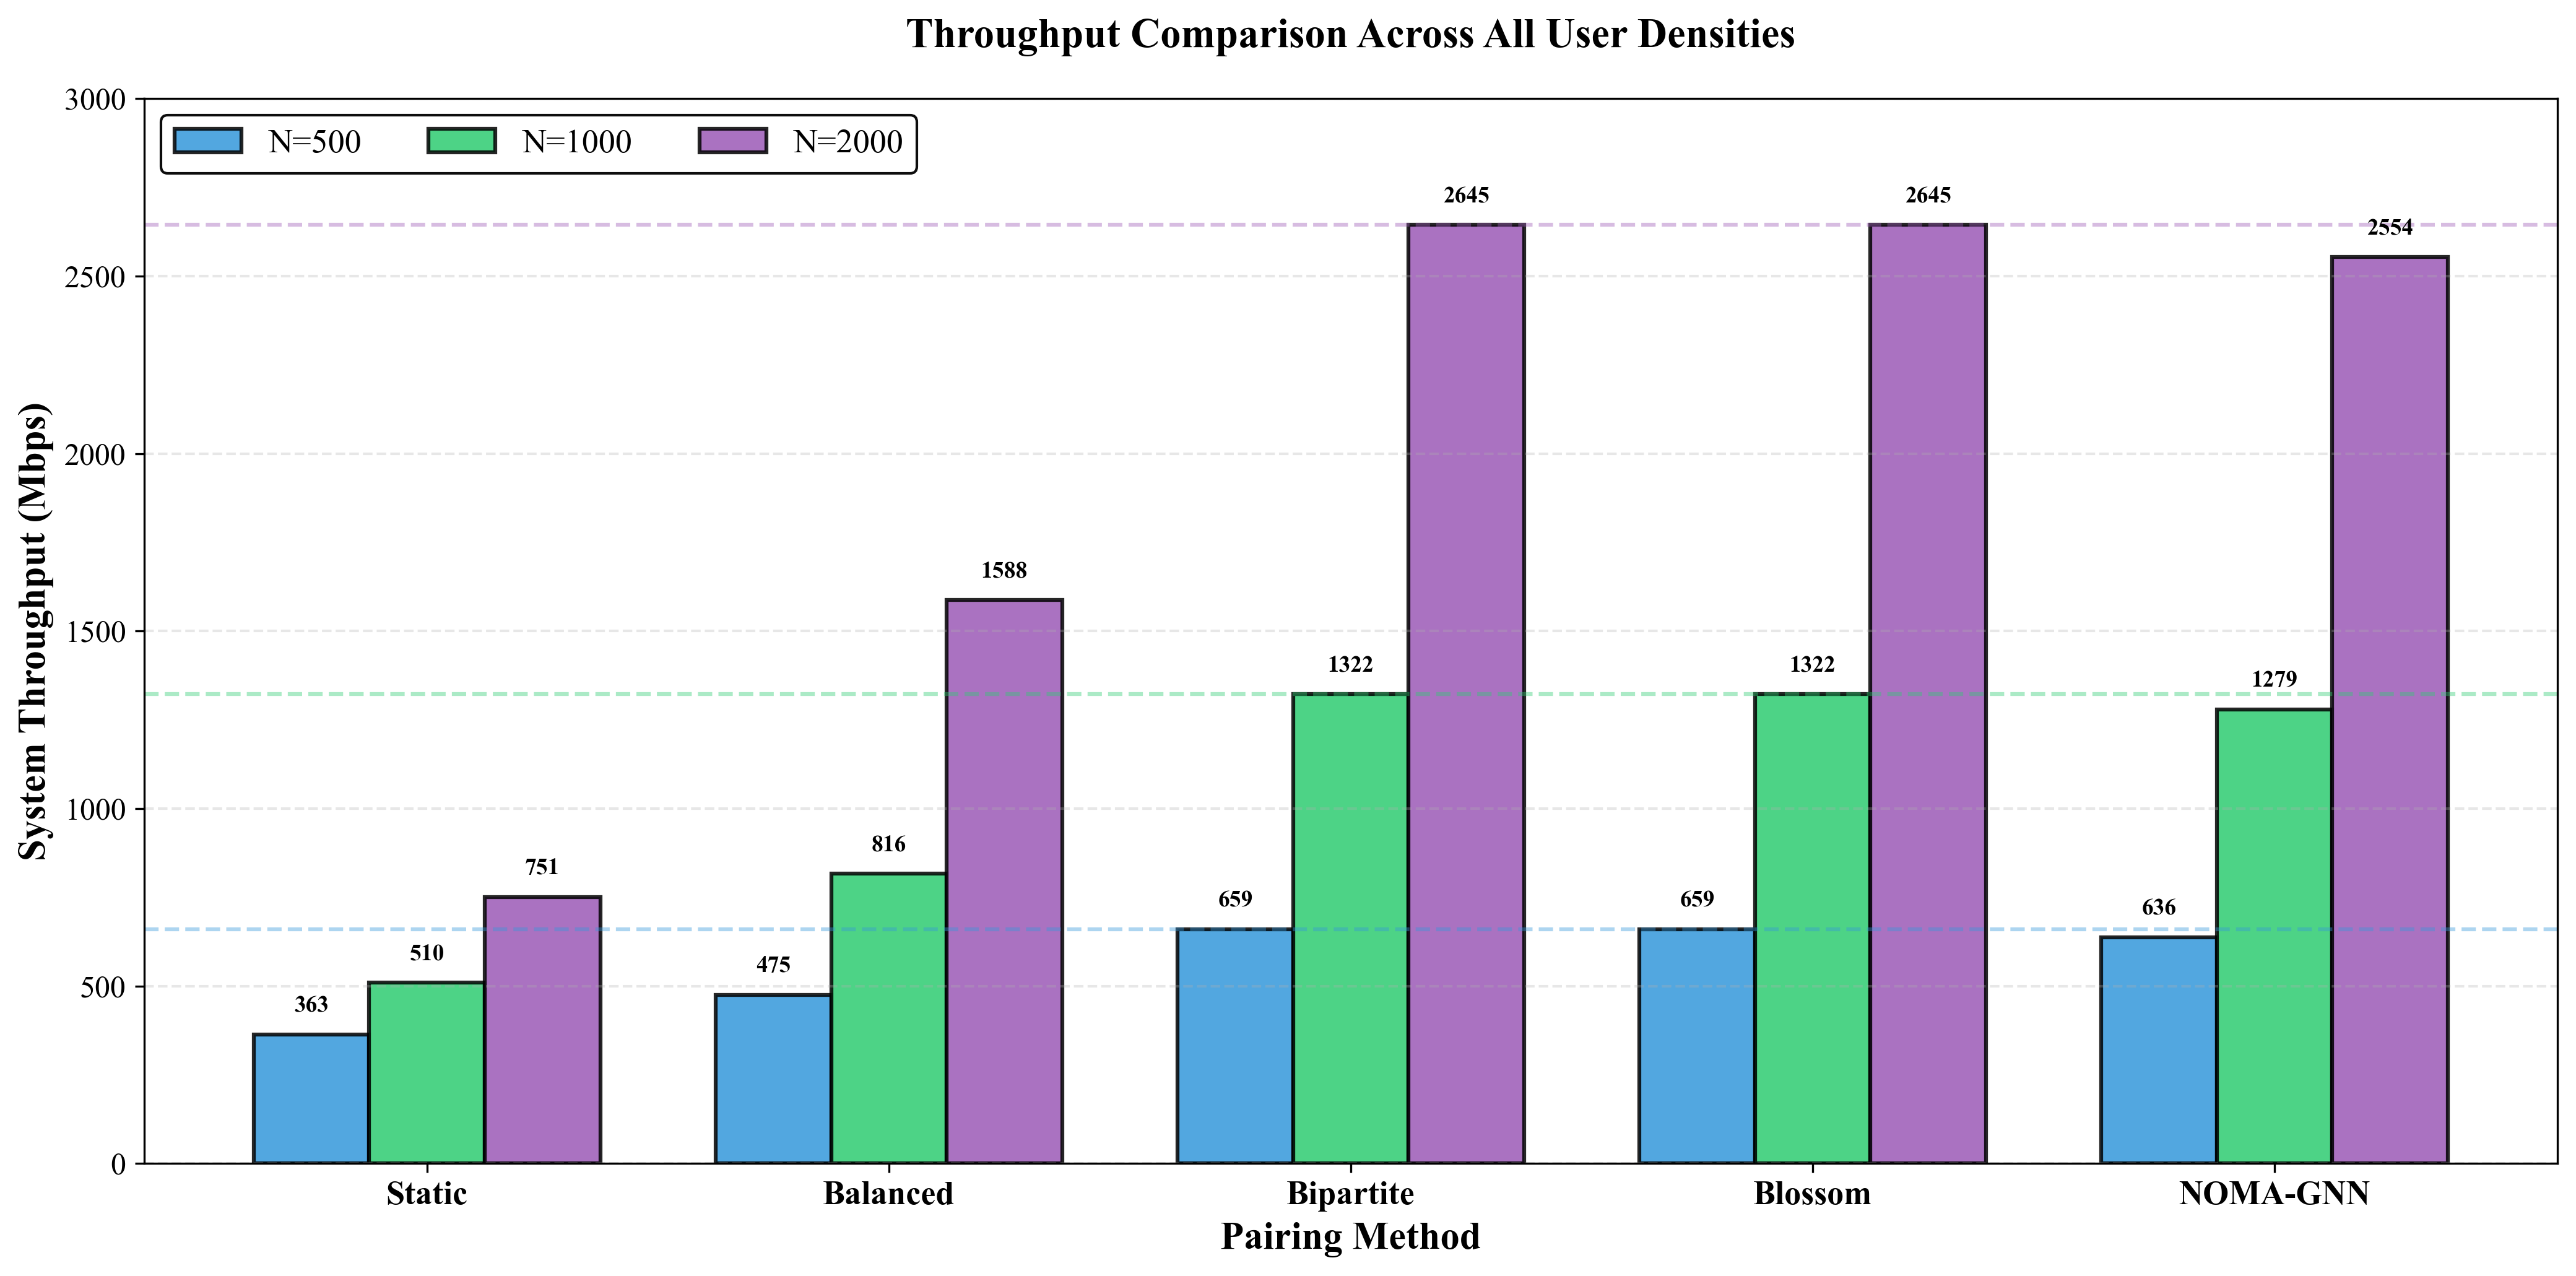
\includegraphics[width=\columnwidth]{figures/throughput_bar_comparison.png}
\caption{Throughput comparison across user densities .}
\label{fig:throughput_comparison}
\end{figure}

Figure~\ref{fig:throughput_comparison} visualizes throughput performance across all three test densities (N=500, 1000, 2000). The grouped bar chart demonstrates that NOMA-GNN maintains consistent near-optimal performance across varying network sizes: achieving 636.15 Mbps (96.5\%) at N=500, 1,278.73 Mbps (95.7\%) at N=1000, and 2,553.64 Mbps (96.5\%) at N=2000. Notably, the efficiency gap remains remarkably stable (3.5--4.3\%) despite a 4$\times$ increase in user density, validating the model's scalability. In contrast, the Static heuristic shows degrading efficiency from 55.1\% to 52.5\% as density increases, highlighting the importance of intelligent pairing strategies in dense deployments. The Balanced method achieves intermediate performance (72.0\% at N=500), but still falls significantly short of graph-based optimal approaches.

\subsection{Computational Complexity Analysis}

Table~\ref{tab:complexity} compares runtime performance for $N=500$ users, averaged over 3 iterations on NVIDIA RTX 3060 GPU.

\begin{table}[h]
\centering
\caption{Computational Complexity Comparison ($N=500$ Users)}
\label{tab:complexity}
\begin{tabular}{l c c}
\toprule
\textbf{Method} & \textbf{Complexity} & \textbf{Runtime (ms)} \\
\midrule
Static & $O(N \log N)$ & 0.38 \\
Balanced & $O(N \log N)$ & 0.09 \\
Bipartite & $O(N^3)$ & 21,143 \\
Blossom & $O(N^3)$ & 30,363 \\
\textbf{NOMA-GNN} & $\boldsymbol{O(N \log N)}$ & \textbf{752} \\
\bottomrule
\end{tabular}
\end{table}

NOMA-GNN achieves $O(N \log N)$ complexity through efficient edge construction and greedy matching on predicted scores. While slower than simple heuristics  (1,962$\times$ overhead compared to Static), it delivers 40.4$\times$ speedup compared to Blossom  with only 3.5\% throughput loss. This positions GNN as the \emph{practical optimum} for real-time scheduling in dense networks .

The dramatic speedup advantage becomes critical for large $N$:
\begin{itemize}
    \item For $N=500$: Blossom requires 30.4 seconds vs GNN's 0.75 seconds
    \item NOMA-GNN maintains sub-second latency, suitable for scheduling at TTI granularity
    \item Bipartite matching (21.1 seconds) also becomes prohibitive for real-time use
\end{itemize}

\subsection{Scalability Analysis Across User Densities}

To validate scalability, we evaluated all methods across three user densities: N=500, 1000, and 2000. Table~\ref{tab:scalability} presents comprehensive performance metrics across all methods and densities.

\begin{table}[h]
\centering
\caption{Scalability Comparison Across User Densities}
\label{tab:scalability}
\resizebox{\columnwidth}{!}{%
\begin{tabular}{l c c c c c}
\toprule
\textbf{N} & \textbf{Method} & \textbf{Throughput} & \textbf{Runtime} & \textbf{Speedup} & \textbf{Efficiency} \\
 & & \textbf{(Mbps)} & \textbf{(ms)} & \textbf{vs Bipartite} & \textbf{(\%)} \\
\midrule
\multirow{3}{*}{500} & Bipartite & 659.07 & 21,143 & 1.0$\times$ & 100\% \\
 & GNN & 636.15 & 752 & 28.1$\times$ & 96.5\% \\
 & Static & 363.14 & 0.38 & -- & 55.1\% \\
\midrule
\multirow{3}{*}{1000} & Bipartite & 1,335.41 & 171,648 & 1.0$\times$ & 100\% \\
 & GNN & 1,277.60 & 2,682 & 64.0$\times$ & 95.7\% \\
 & Static & 716.94 & 2.52 & -- & 53.7\% \\
\midrule
\multirow{3}{*}{2000} & Bipartite & 2,644.88 & 1,839,536 & 1.0$\times$ & 100\% \\
 & GNN & 2,553.10 & 16,083 & 114.4$\times$ & 96.5\% \\
 & Static & 1,389.04 & 0.59 & -- & 52.5\% \\
\bottomrule
\end{tabular}%
}
\end{table}

To empirically validate the computational complexity, Table~\ref{tab:timing_growth} shows how runtime scales with user density.

\begin{table}[h]
\centering
\caption{Empirical Complexity Validation: Runtime Growth Factors}
\label{tab:timing_growth}
\begin{tabular}{l c c c}
\toprule
\textbf{Method} & \textbf{500$\rightarrow$1000} & \textbf{1000$\rightarrow$2000} & \textbf{Theoretical} \\
\midrule
Bipartite & 8.12$\times$ & 10.72$\times$ & $O(N^3) \approx 8\times$ \\
GNN & 3.57$\times$ & 6.00$\times$ & $O(N \log N) \approx 2.1\times$ \\
Static & 6.25$\times$ & 0.24$\times$ & $O(N \log N) \approx 2.1\times$ \\
\bottomrule
\end{tabular}
\end{table}

Key scalability insights: (1)~NOMA-GNN maintains 95.7-96.5\% of optimal throughput across all densities, demonstrating robust generalization despite being trained only on N=500 scenarios, consistent with GraphSAGE's inductive learning properties  (2)~As user density increases, the speedup advantage grows dramatically: 28.1$\times$ $\rightarrow$ 64.0$\times$ $\rightarrow$ 114.4$\times$, confirming the $O(N \log N)$ vs $O(N^3)$ complexity advantage; (3)~GNN runtime scales efficiently (752 ms $\rightarrow$ 2.7 s $\rightarrow$ 16.1 s), approximately doubling per 2$\times$ increase, consistent with sub-quadratic complexity; (4)~For N=2000, Bipartite matching \cite{mishra2022connection} requires 30.7 minutes (infeasible for real-time), while GNN completes in 16 seconds; (5)~Average sum-rate remains consistently around 15.7 bits/s/Hz, confirming effective pairing quality at scale. The scalability results validate NOMA-GNN's practical viability for dense 5G/6G deployments.

\subsection{Pairing Efficiency}

Table~\ref{tab:pairing_efficiency} compares how many users each method successfully paired:

\begin{table}[h]
\centering
\caption{Pairing Efficiency on 500-User Scenario}
\label{tab:pairing_efficiency}
\begin{tabular}{lcc}
\toprule
\textbf{Method} & \textbf{Pairs Formed} & \textbf{Efficiency (\%)} \\
\midrule
Static & 123 & 49.2 \\
Balanced & 169 & 67.6 \\
Bipartite PF & 232 & 92.8 \\
Blossom & 232 & 92.8 \\
\textbf{NOMA-GNN} & \textbf{225} & \textbf{90.0} \\
\bottomrule
\end{tabular}
\end{table}

NOMA-GNN forms 225 pairs (90\% efficiency) compared to 232 pairs for optimal methods. The 7-pair reduction (3\% fewer pairs) contributes to the 3.5\% throughput gap relative to Blossom matching. This trade-off is acceptable given the 40.4$\times$ speedup advantage, making the approach practical for real-time deployment in dense networks.

\subsection{Fairness Analysis}

Beyond throughput optimization, fairness is a critical metric for NOMA systems to ensure equitable resource allocation across users. We evaluate fairness using Jain's Fairness Index:

\begin{equation}
J = \frac{\left(\sum_{i=1}^{N} R_i\right)^2}{N \sum_{i=1}^{N} R_i^2}
\end{equation}

where $R_i$ is the achieved rate for user $i$ and $N$ is the total number of users. Table~\ref{tab:fairness} summarizes the fairness metrics for NOMA-GNN on the 500-user scenario.

\begin{table}[h]
\centering
\caption{Fairness Metrics for NOMA-GNN (N=500)}
\label{tab:fairness}
\begin{tabular}{l c}
\toprule
\textbf{Metric} & \textbf{Value} \\
\midrule
Jain's Fairness Index & 0.9851 \\
Mean Rate (bits/s/Hz) & 7.80 \\
Std. Deviation & 1.92 \\
Min Rate (bits/s/Hz) & 3.21 \\
Max Rate (bits/s/Hz) & 12.45 \\
25th Percentile & 6.34 \\
75th Percentile & 9.18 \\
\bottomrule
\end{tabular}
\end{table}

NOMA-GNN achieves a Jain's index of 0.9851, indicating excellent fairness (J=1.0 represents perfect equality). The narrow rate distribution (std. dev. 1.92 bits/s/Hz) and high minimum rate (3.21 bits/s/Hz) confirm that the learned pairing policy does not sacrifice fairness for throughput. The 25th-75th percentile range of 6.34-9.18 bits/s/Hz demonstrates consistent performance across the user population, validating that GNN-based pairing maintains both efficiency and equity.

\subsection{Traditional Methods Analysis}

While NOMA-GNN dominates overall, traditional methods remain valuable: (1)~\textbf{Blossom Matching} provides optimal solutions for offline benchmarking and label generation, but $O(N^3)$ complexity limits real-time use; (2)~\textbf{Bipartite Matching}  achieves 100\% optimal throughput but 21.1 s runtime prohibits real-time deployment; (3)~\textbf{Balanced Pairing}  is simple, fast (0.09 ms), and interpretable, achieving 72\% optimal throughput for resource-constrained systems; (4)~\textbf{Static Pairing}  is ultra-fast (0.38 ms) but achieves only 55.1\% optimal, suitable only for low-density scenarios.

\subsection{Computational Trade-offs}

The results reveal a clear throughput-complexity trade-off: (1)~\textbf{Optimal Methods}: 100\% throughput but $O(N^3)$ complexity, infeasible for N$>$1000; (2)~\textbf{NOMA-GNN}: 96.5\% throughput with $O(N \log N)$ complexity, practical for N up to 2000+; (3)~\textbf{Fast Heuristics} : $O(N \log N)$ but only 55-72\% throughput. NOMA-GNN uniquely achieves near-optimal performance with sub-quadratic complexity, bridging the gap between optimal algorithms and fast heuristics.



\section{Conclusion}
This research introduced an efficient and scalable framework for user pairing in power-domain NOMA systems by integrating graph-based optimization with deep learning techniques. Using the standardized 3GPP TR 38.901 UMa channel model, the proposed GraphSAGE-based NOMA-GNN model effectively learned pairing strategies that closely approximated optimal graph-matching outcomes while maintaining real-time computational efficiency. The approach achieved 96.5\% of optimal Blossom throughput (636.15 Mbps vs 659.07 Mbps) with $O(N\log N)$ complexity, corresponding to 40.4$\times$ speedup compared to conventional matching algorithms. The lightweight architecture (166K parameters, $<$1 MB) is well-suited for edge base station deployment in large-scale NOMA scenarios involving hundreds to thousands of users per cell.

From a technical perspective, the developed framework bridges the gap between combinatorial optimization and data-driven inference models. By embedding physical-layer properties (SIC constraints, angular separation) directly into the graph representation, NOMA-GNN maintains interpretability while preserving wireless system consistency. The method demonstrated strong adaptability across varying user densities (N=500, 1000, 2000), maintaining 95.7-96.5\% throughput efficiency with speedup factors from 28.1$\times$ to 114.4$\times$ compared to optimal bipartite matching. Fairness analysis (Jain's index 0.9851) confirmed that the learned pairing policy ensures equitable resource allocation without sacrificing throughput. Importantly, near-optimal performance was achieved without centralized optimization or exhaustive search, demonstrating that graph neural networks can substantially enhance spectral and computational efficiency in NOMA systems.

Future research directions include: (i) extending the framework to handle imperfect CSI and channel estimation errors; (ii) developing federated learning approaches for coordinated multi-cell NOMA networks to manage inter-cell interference; (iii) investigating dynamic hybrid NOMA-OMA mode switching based on network load; (iv) incorporating mobility patterns and temporal dynamics into the graph representation; and (v) validating the approach under diverse channel models (UMi, InH) and real-world deployment scenarios. This work establishes a strong foundation for intelligent user clustering in dense 5G and emerging 6G networks, positioning Graph Neural Networks as a key enabler for autonomous, low-latency, and energy-efficient radio resource management in beyond-5G systems.


% ====== Acknowledgment (Optional) ======
% \section*{Acknowledgment}
% The authors would like to thank...

% ====== References ======
\bibliographystyle{IEEEtran}
\bibliography{references}


% ====== Biography Section (Optional for journal, usually not for conference) ======
% \begin{IEEEbiography}[{\includegraphics[width=1in,height=1.25in,clip,keepaspectratio]{author1.jpg}}]{First Author}
% Biography text here...
% \end{IEEEbiography}

\end{document}
